\documentclass[12pt]{article}
\usepackage{fontspec}
\usepackage{polyglossia}
\setmonofont{Courier New}
\setmainlanguage{farsi}
\setotherlanguage{english}
\newfontfamily\persianfont[Script=Arabic]{XBZar}
\usepackage{graphicx}
\usepackage{geometry}
\usepackage{hyperref}
\geometry{a4paper, margin=2.5cm}
\usepackage{setspace}
\usepackage{url}
\onehalfspacing
\usepackage{titling}
\usepackage{float}
\usepackage{etoolbox}
\usepackage[backend=biber,style=numeric,sorting=none]{biblatex}
%%%%%%%%%%%%%%%%%%%%%%%%%%%%%%%%%%%%%%%%%%%%%%%%%%%%%%%%%%%%%%%%%%%%%%%%%%%%%
\makeatletter
\newcommand{\persiandigit}[1]{%
	\ifcase#1 ۰\or ۱\or ۲\or ۳\or ۴\or ۵\or ۶\or ۷\or ۸\or ۹\fi
}
\DeclareFieldFormat{labelnumber}{\persiandigit{#1}}
\makeatother
%%%%%%%%%%%%%%%%%%%%%%%%%%%%%%%%%
\newcommand{\persianordinal}[1]{%
	\ifcase#1
	\or اول%
	\or دوم%
	\or سوم%
	\or چهارم%
	\or پنجم%
	\or ششم%
	\or هفتم%
	\or هشتم%
	\or نهم%
	\or دهم%
	\or یازدهم%
	\or دوازدهم%
	\or سیزدهم%
	\or چهاردهم%
	\or پانزدهم%
	\or شانزدهم%
	\or هفدهم%
	\or هجدهم%
	\or نوزدهم%
	\or بیستم%
	\else #1\fi
}

\newcommand{\persianordinalpage}{\persianfont\persianordinal{\value{page}}}


%%%%%%%%%%%%%%%%%%%%%%%%%%%%%%%%%%%%%%%%%%%%%%%%%%%%%%%%%%%%%%%%%%%%%%%%%%%%%
\begin{filecontents}{\jobname.bib}
	@online{a1,
		url = {https://en.wikipedia.org/wiki/Dynamic_Host_Configuration_Protocol}
	}
	@online{a2,
		url = {https://wiki.wireshark.org/TLS}
	}
	@online{a3,
		url = {https://wiki.wireshark.org/RTP_statistics}
	}
	
\end{filecontents}

\addbibresource{\jobname.bib}

\defbibheading{bibliography}[]{%
	\begin{RTL}
		\section*{مراجع}
	\end{RTL}
}

%%%%%%%%%%%%%%%%%%%%%%%%%%%%%%%%%%%%%%%%%%%%%%%%%%%%%%%%%%%%%%%%%%%%%%%%%%%%%

\begin{document}
	
	% ==============================
	% Title Page
	% ==============================
	\begin{titlepage}
		\centering
		\vspace*{1cm}
		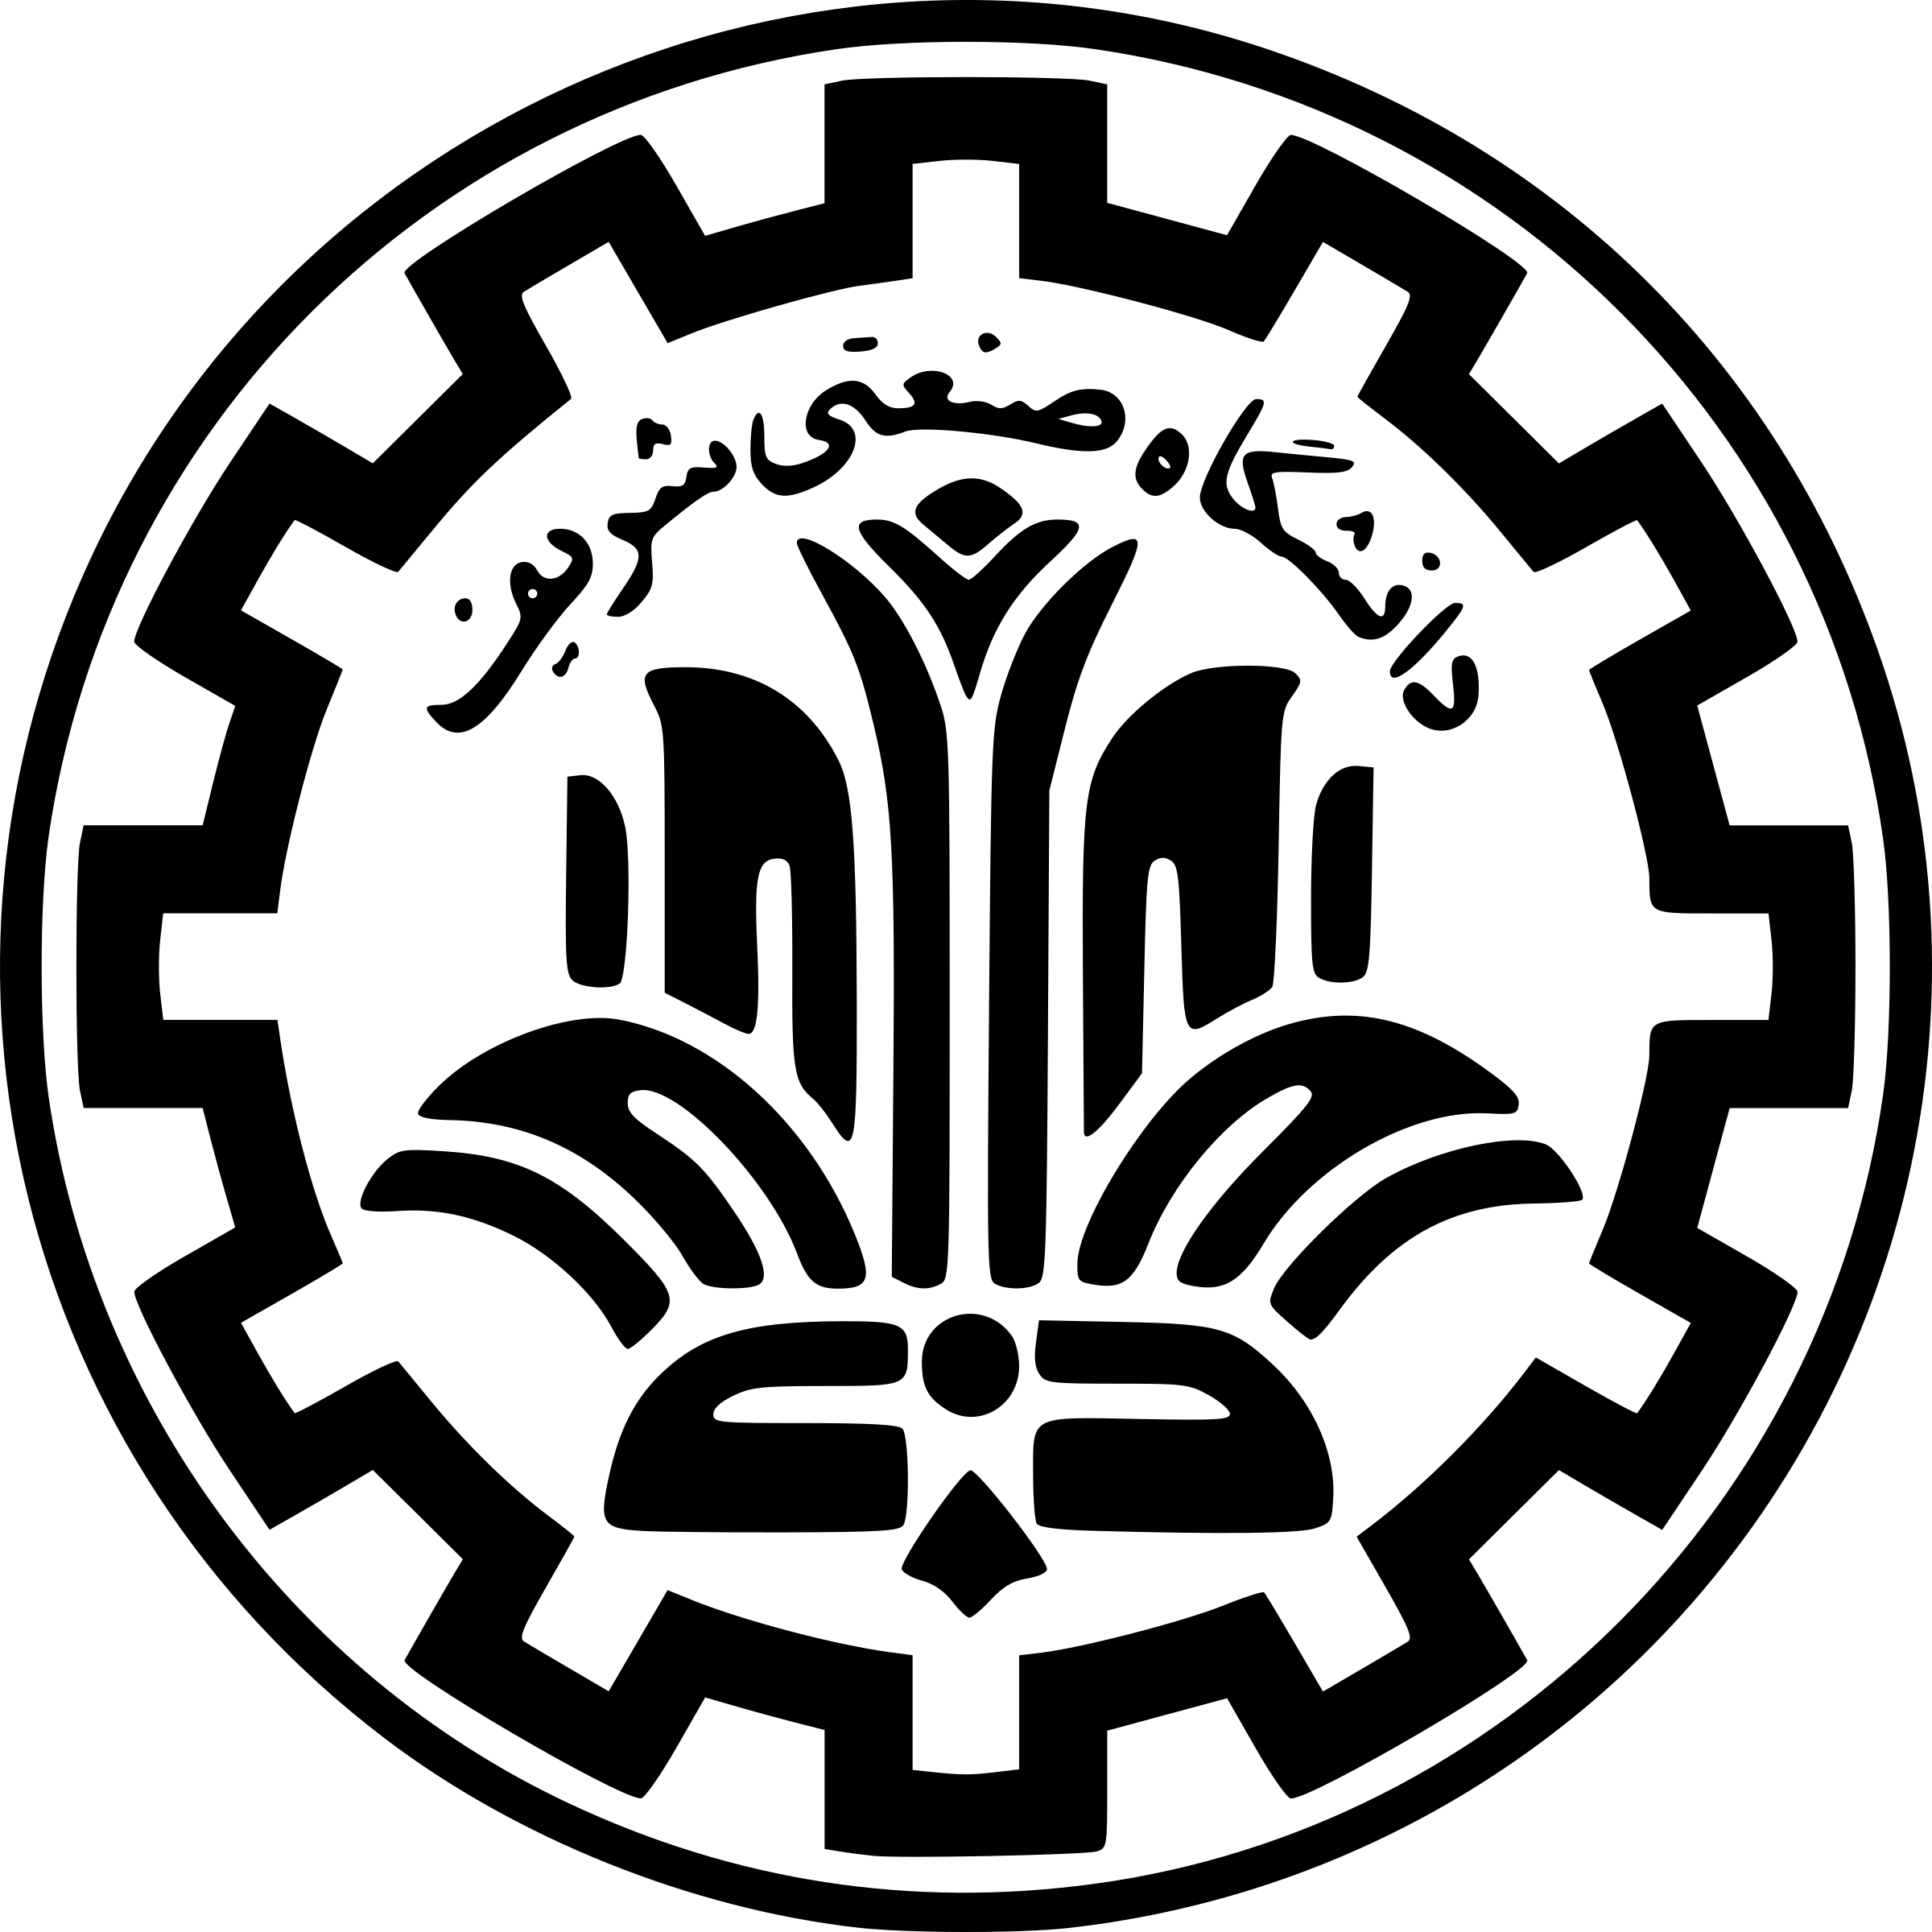
\includegraphics[width=4cm]{sharif.png}\\[1.5cm]
		{\Large\textbf{دانشگاه صنعتی شریف}}\\[0.5cm]
		{\large\textbf{دانشکدهٔ مهندسی کامپیوتر}}\\[1.5cm]
		{\Huge\textbf{گزارش کار آزمایشگاه}}\\[0.5cm]
		{\LARGE\textbf{آزمایشگاه شبکه‌های کامپیوتری}}\\[2cm]
		
		\textbf{گزارش آزمایش شماره ۷}\\
		(آشنایی با \textenglish{DHCP}‬‬)
		
		\vfill
		\begin{tabular}{rl}
			\textbf{شمارهٔ گروه:} & ۴ \\
			\textbf{گروه:} &
			ارشیا یوسف‌نیا (۴۰۱۱۱۰۴۱۵) \\
			& محمد‌فرحان بهرامی (۴۰۱۱۰۵۷۲۹) \\
			& امیرمهدی دارایی (۹۹۱۰۵۴۳۱) \\
			\textbf{استاد درس:} & دکتر صفایی \\
			\textbf{تاریخ:} & تابستان ۱۴۰۴ \\
		\end{tabular}
	\end{titlepage}
	
	% ==============================
	% Persian Ordinal Page Numbering
	% ==============================
	\clearpage
	\setcounter{page}{1}
	\renewcommand{\thepage}{\persianordinalpage}
	
	\tableofcontents
	\clearpage
	\listoffigures
	%\clearpage
	%\listoftables
	
	% ==============================
	% Switch to Persian Digits (۱, ۲, ۳, ...)
	% ==============================
	\clearpage
	\setcounter{page}{1}
	\pagenumbering{arabic}
	\renewcommand{\thepage}{\persianfont\arabic{page}}
	
	
	% ==============================
	% Main Content
	% ==============================
	\section{مقدمه}
	در این آزمایش ۳ سناریو مختلف استفاده از \textenglish{DHCP} را مطابق فیلم داده شده بررسی می‌کنیم \cite{a1}. بعضی جزییات مانند آدرس‌ها و موارد مربوط به شبکه در شکل‌های خوانا آورده شده است و در متن دوباره تکرار نشده است.
	
	\section{سناریو ۱}
	مطابق شکل \ref{1:1} در ابتدا دستگاه‌های مورد نیاز را میاوریم و به هم وصل می‌کنیم. در ادامه در \textenglish{Light Weight Access Point} ماژول \textenglish{ACCESS POINT POWER ADAPTER} را مانند شکل \ref{1:2} اضافه می‌کنیم. گام بعدی تخصیص آدرس \textenglish{ip} مناسب به مسیریاب است. این مورد در شکل \ref{1:3} آمده است. اکنون باید به سرور خود آدرس \textenglish{Default Gateway} و آدرس سرویس \textenglish{DNS} را طبق شکل \ref{1:4} اضافه کنیم. در ادامه باید سرور روشن باشد و آدرس مناسب در شبکه داشته باشد. این کار در شکل \ref{1:5} انجام شده است. گام بعد راه‌اندازی سرویس \textenglish{DHCP} با استخر‌ها و تنظیمات درست است. شکل \ref{1:6} این فرآیند را نشان می‌دهد. حالا وارد دستگاه‌های \textenglish{PC} شبکه می‌شویم و در بخش آدرس آن‌ها حالت خودکار با \textenglish{DHCP} را انتخاب می‌کنیم و آدرس‌ها با موفقیت تخصیص داده می‌شود. در شکل \ref{1:7} نتیجه اینکار روی یک دستگاه آمده است. همچنین شکل \ref{1:8} شبیه‌سازی دیداری حرکت بسته‌ها را نشان می‌دهد. در نهایت شکل \ref{1:9} دریافت درست آدرس را در یک دستگاه دیگر در شبکه نشان می‌دهد.
	
	\begin{figure}[H]
		\centering
		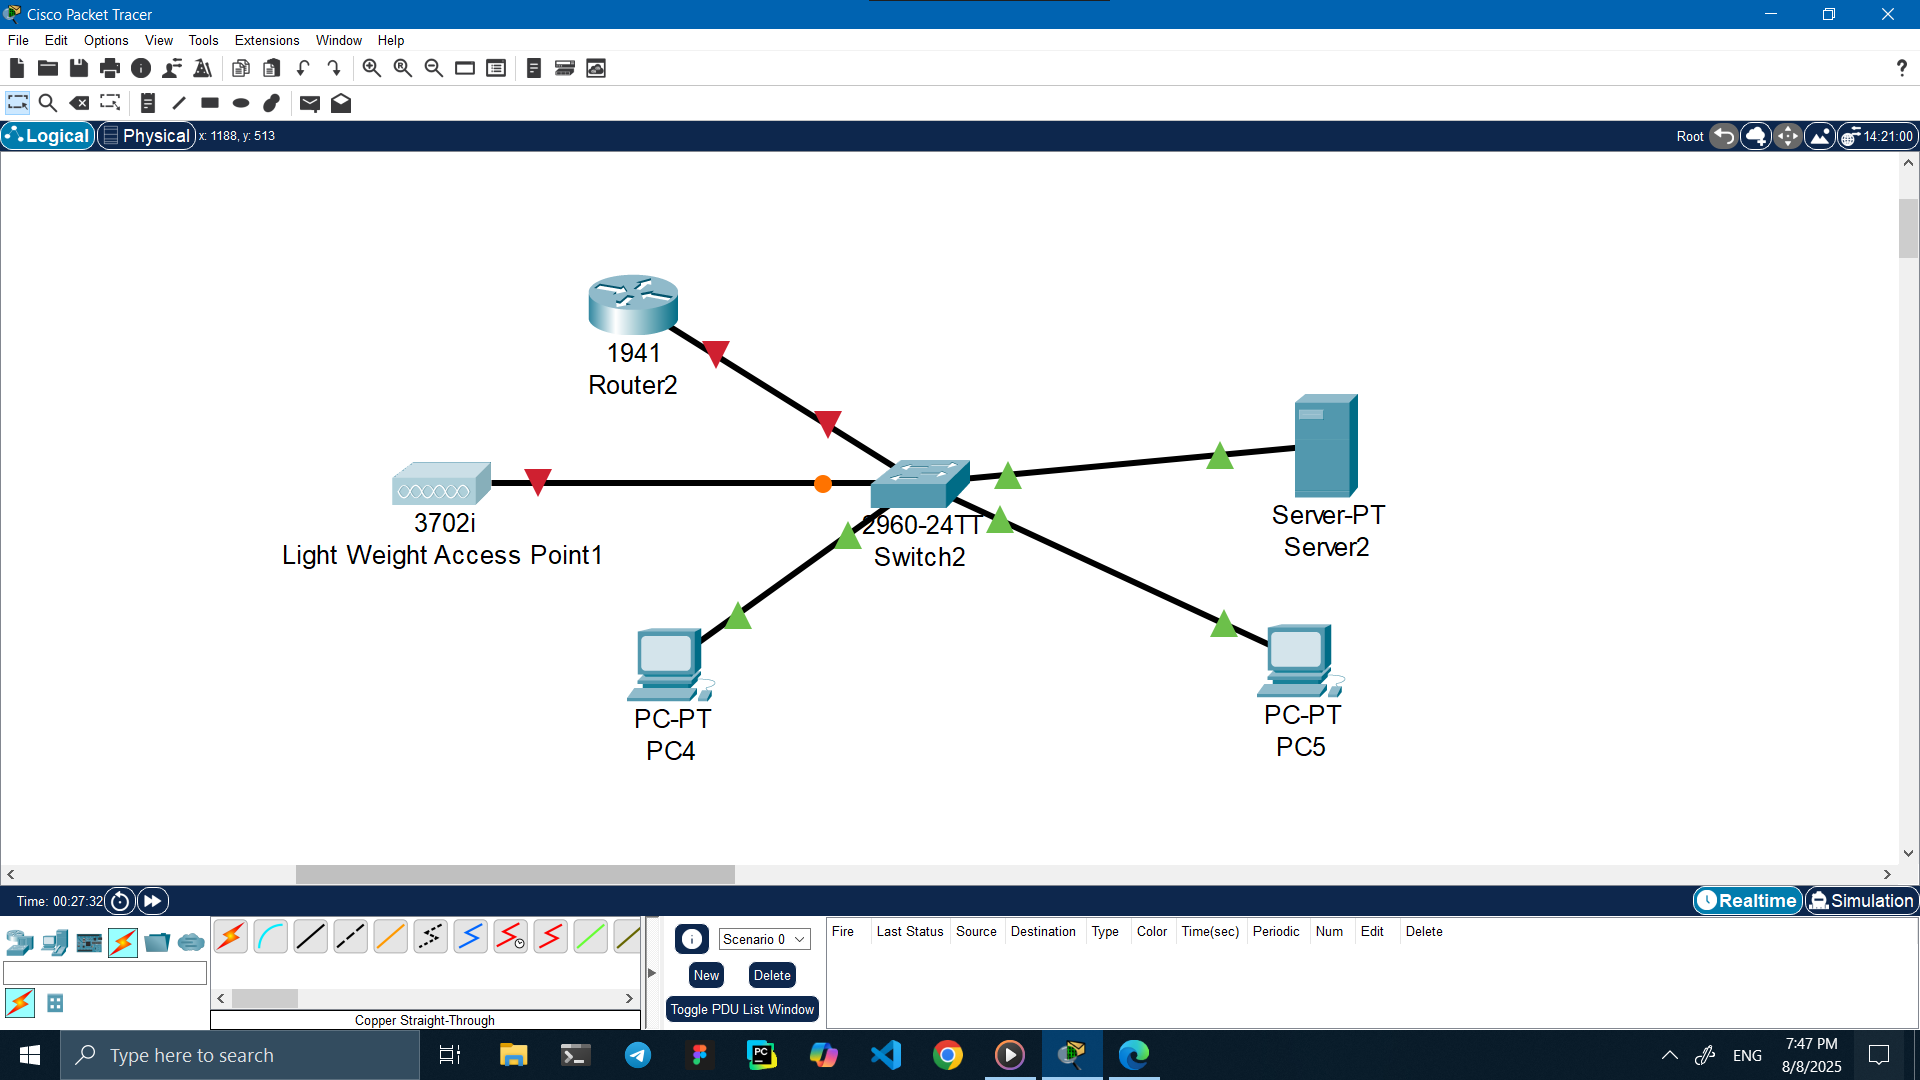
\includegraphics[width=\textwidth]{resources/scenario1-1.png}
		\caption{اضافه کردن دستگاه‌ها و اتصالات سناریو ۱}
		\label{1:1}
	\end{figure}
	\begin{figure}[H]
		\centering
		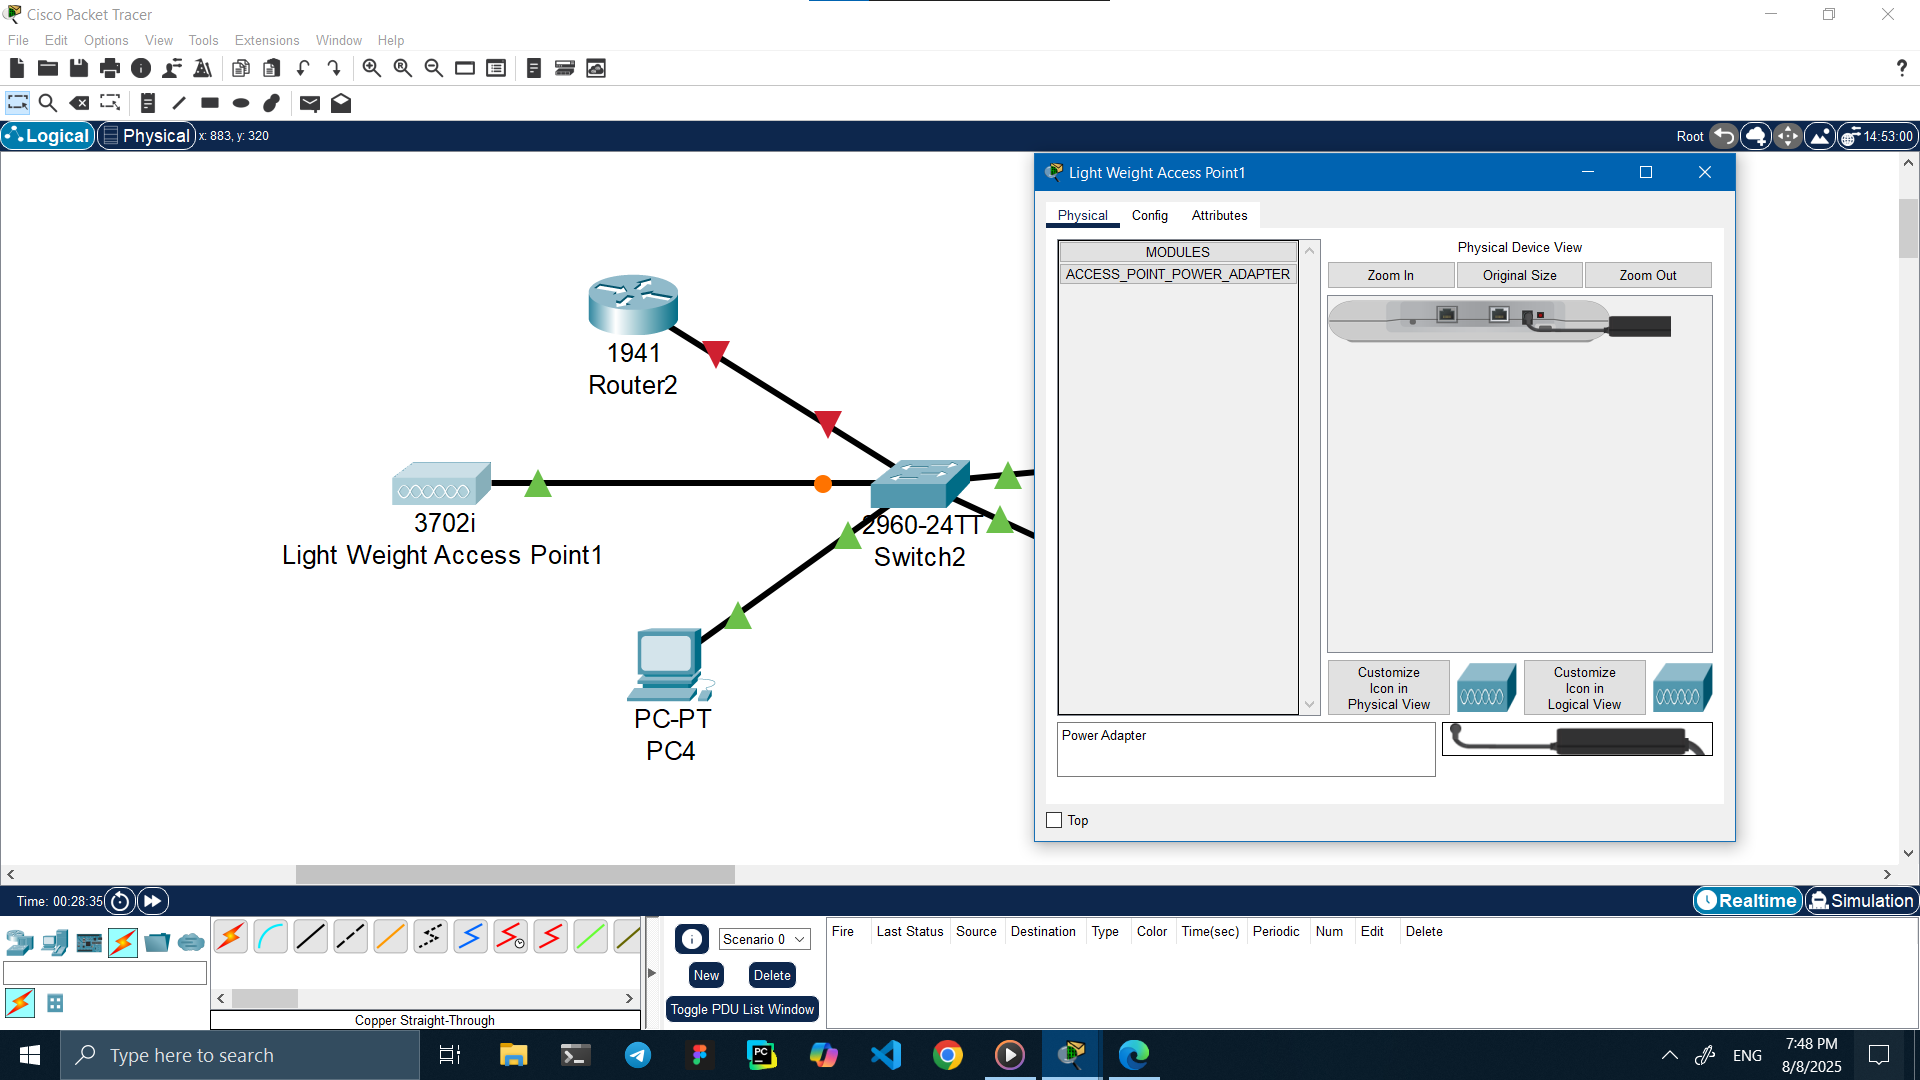
\includegraphics[width=\textwidth]{resources/scenario1-2.png}
		\caption{تنظیم ماژول‌های مورد نیاز \textenglish{Light Weight Access Point}}
		\label{1:2}
	\end{figure}
	\begin{figure}[H]
		\centering
		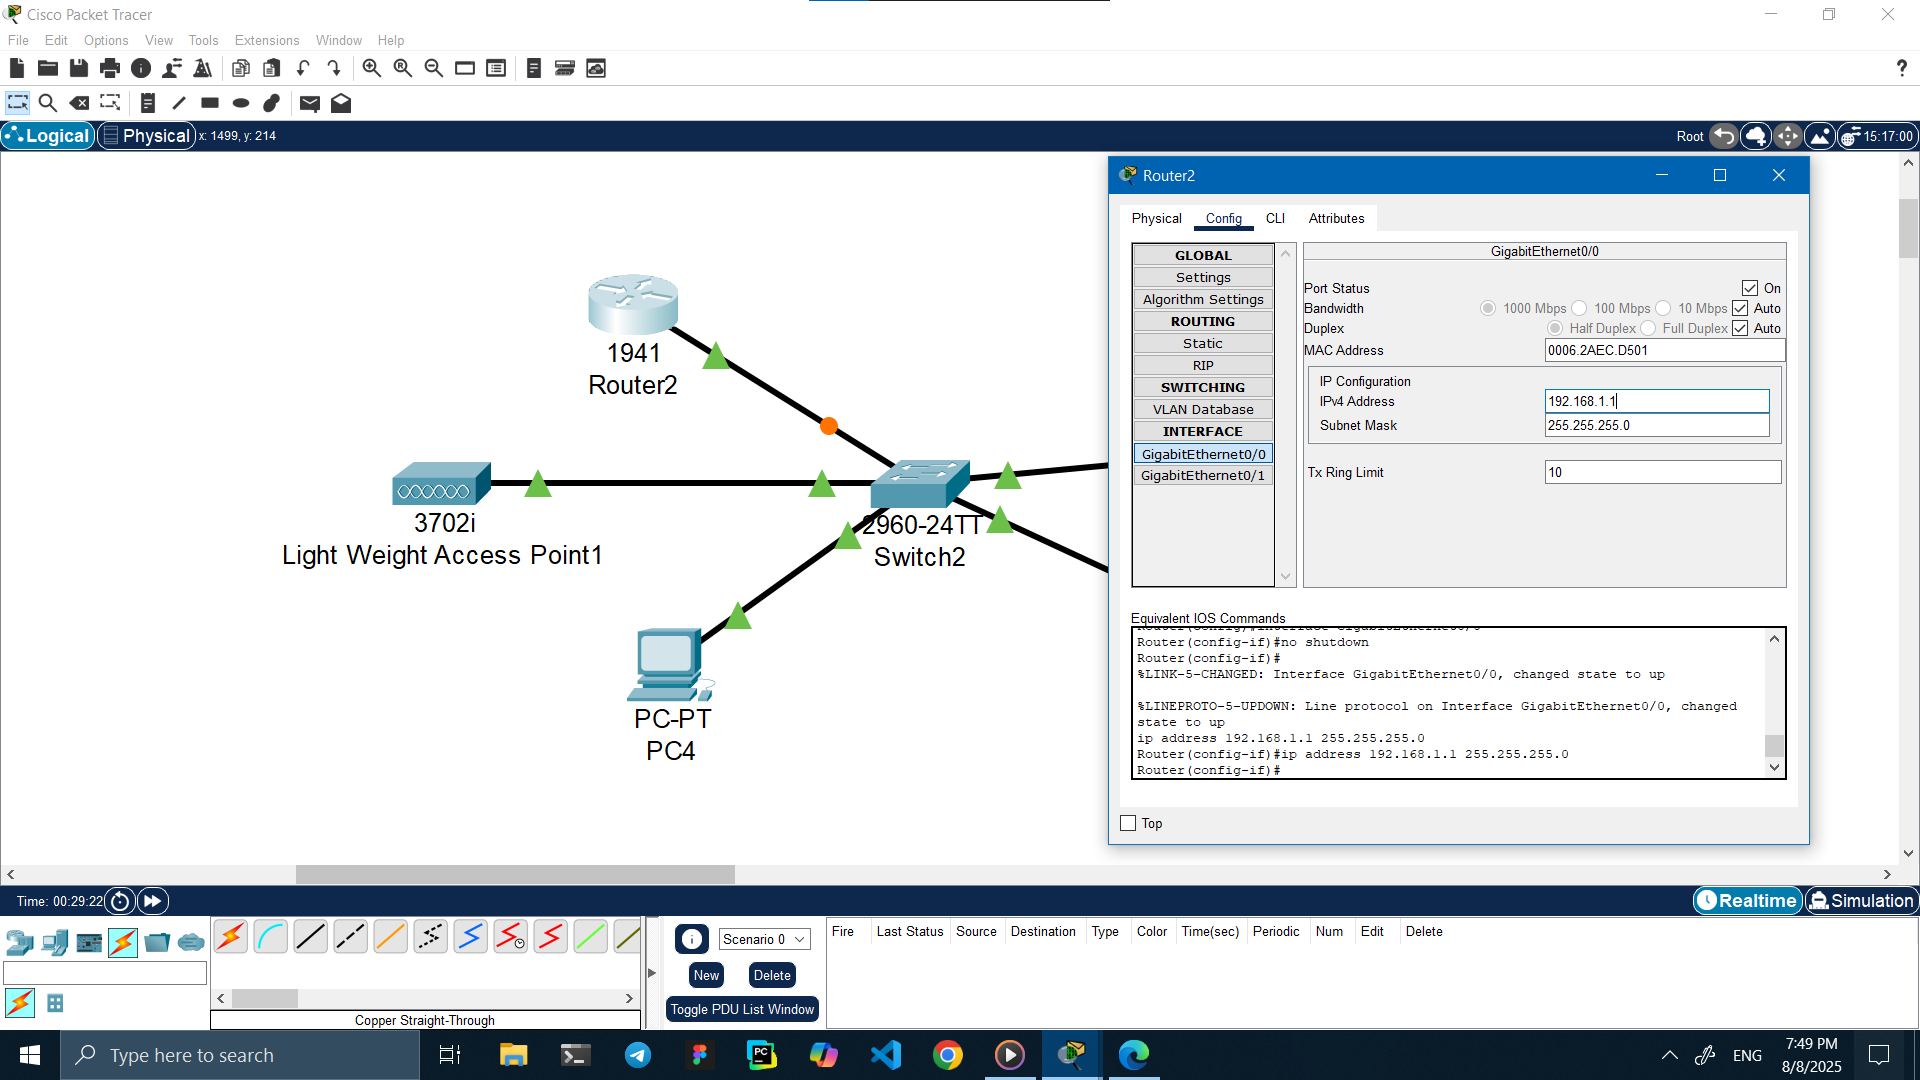
\includegraphics[width=\textwidth]{resources/scenario1-3.png}
		\caption{تخصیص آدرس \textenglish{ip} مناسب به \textenglish{Router}}
		\label{1:3}
	\end{figure}
	\begin{figure}[H]
		\centering
		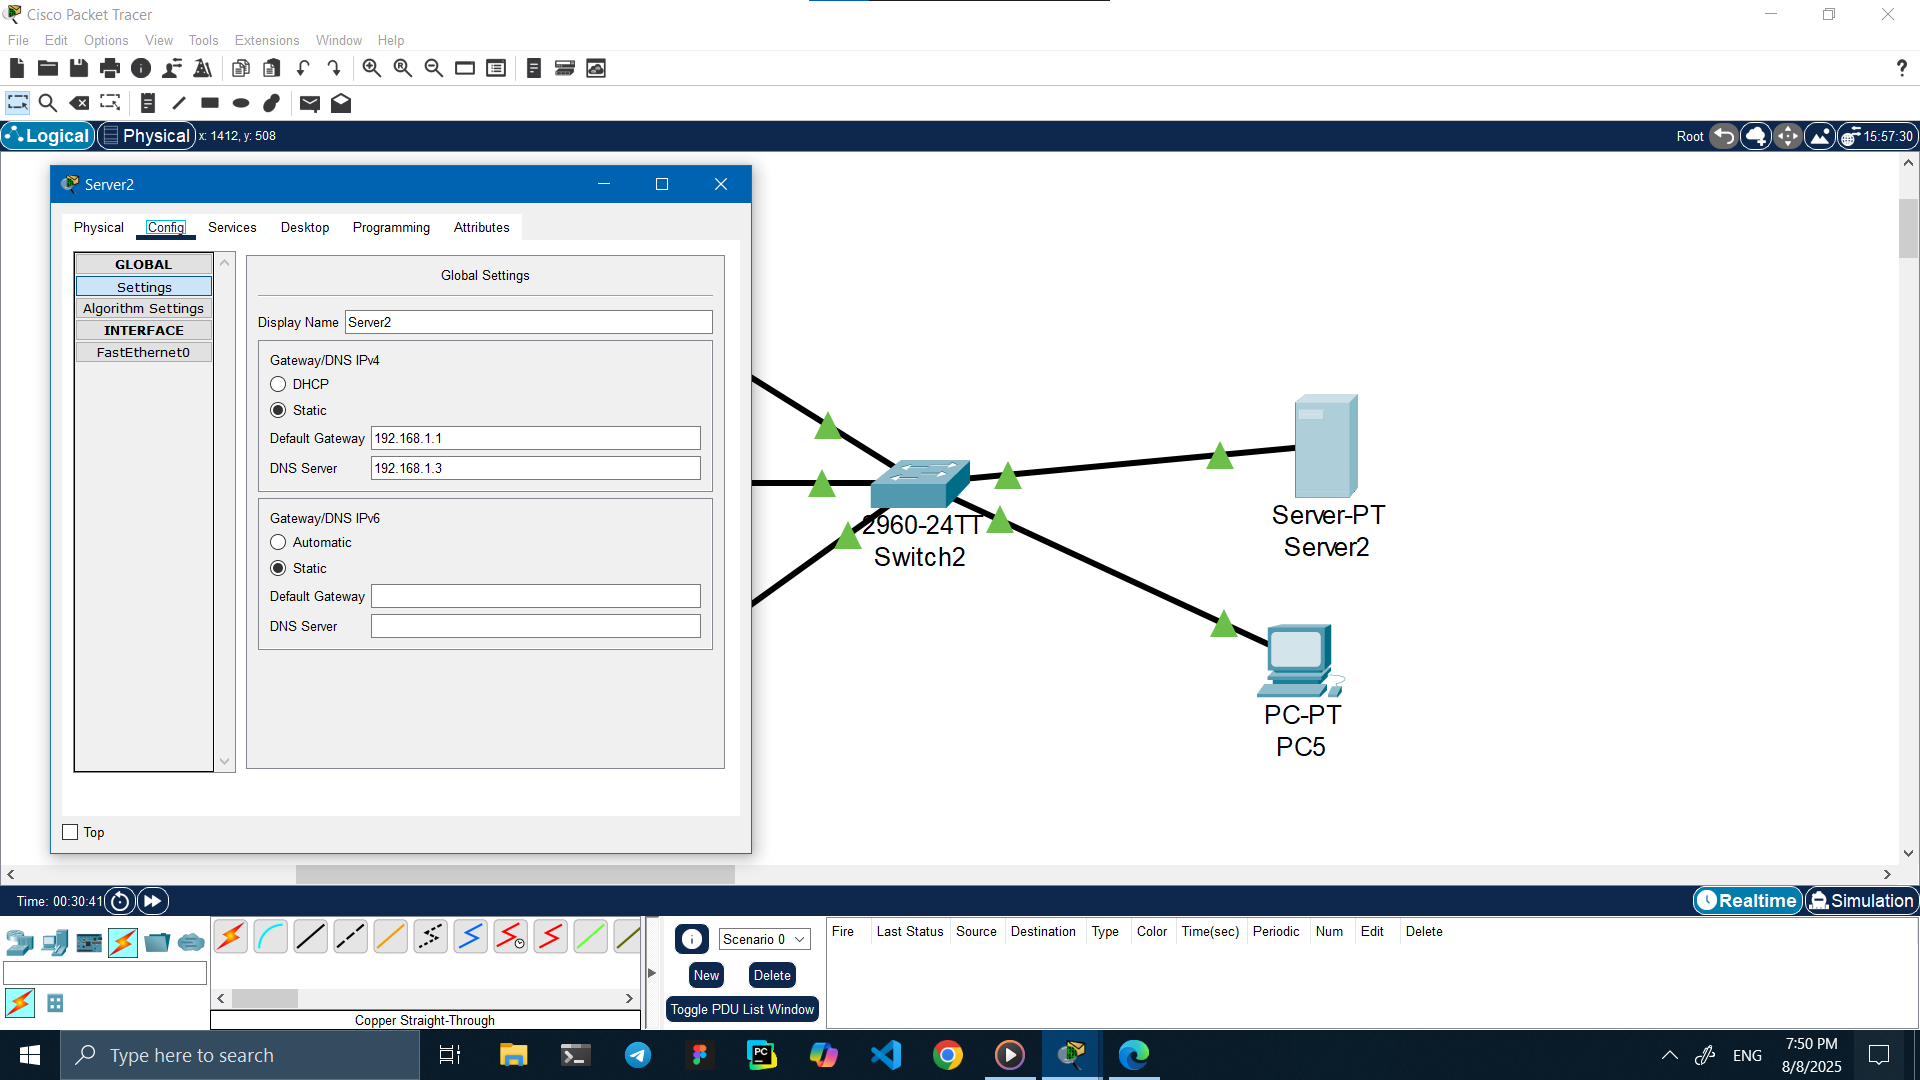
\includegraphics[width=\textwidth]{resources/scenario1-4.png}
		\caption{اضافه کردن \textenglish{Default Gateway} و \textenglish{DNS Server} در تنظیمات سرور}
		\label{1:4}
	\end{figure}
	\begin{figure}[H]
		\centering
		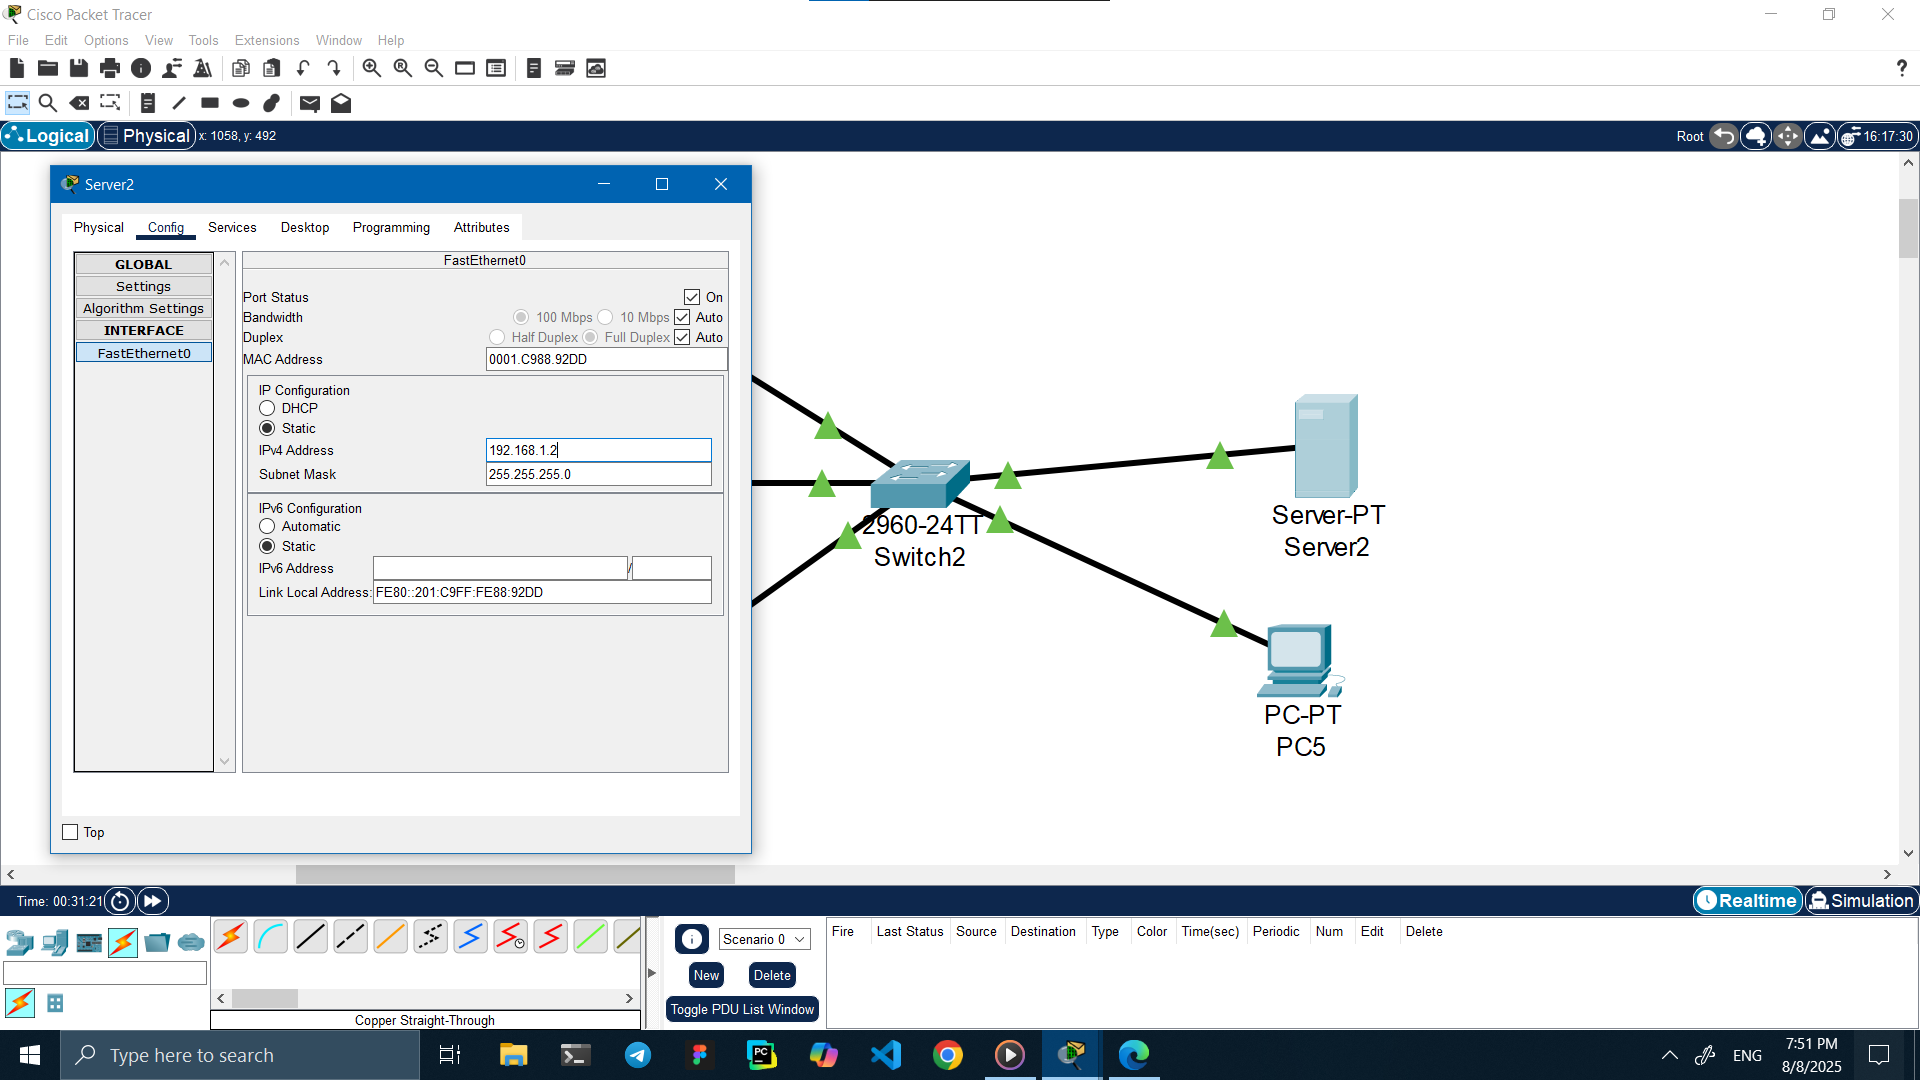
\includegraphics[width=\textwidth]{resources/scenario1-5.png}
		\caption{تنظیم آدرس \textenglish{ip} سرور و اطمینان از روشن بودن آن}
		\label{1:5}
	\end{figure}
	\begin{figure}[H]
		\centering
		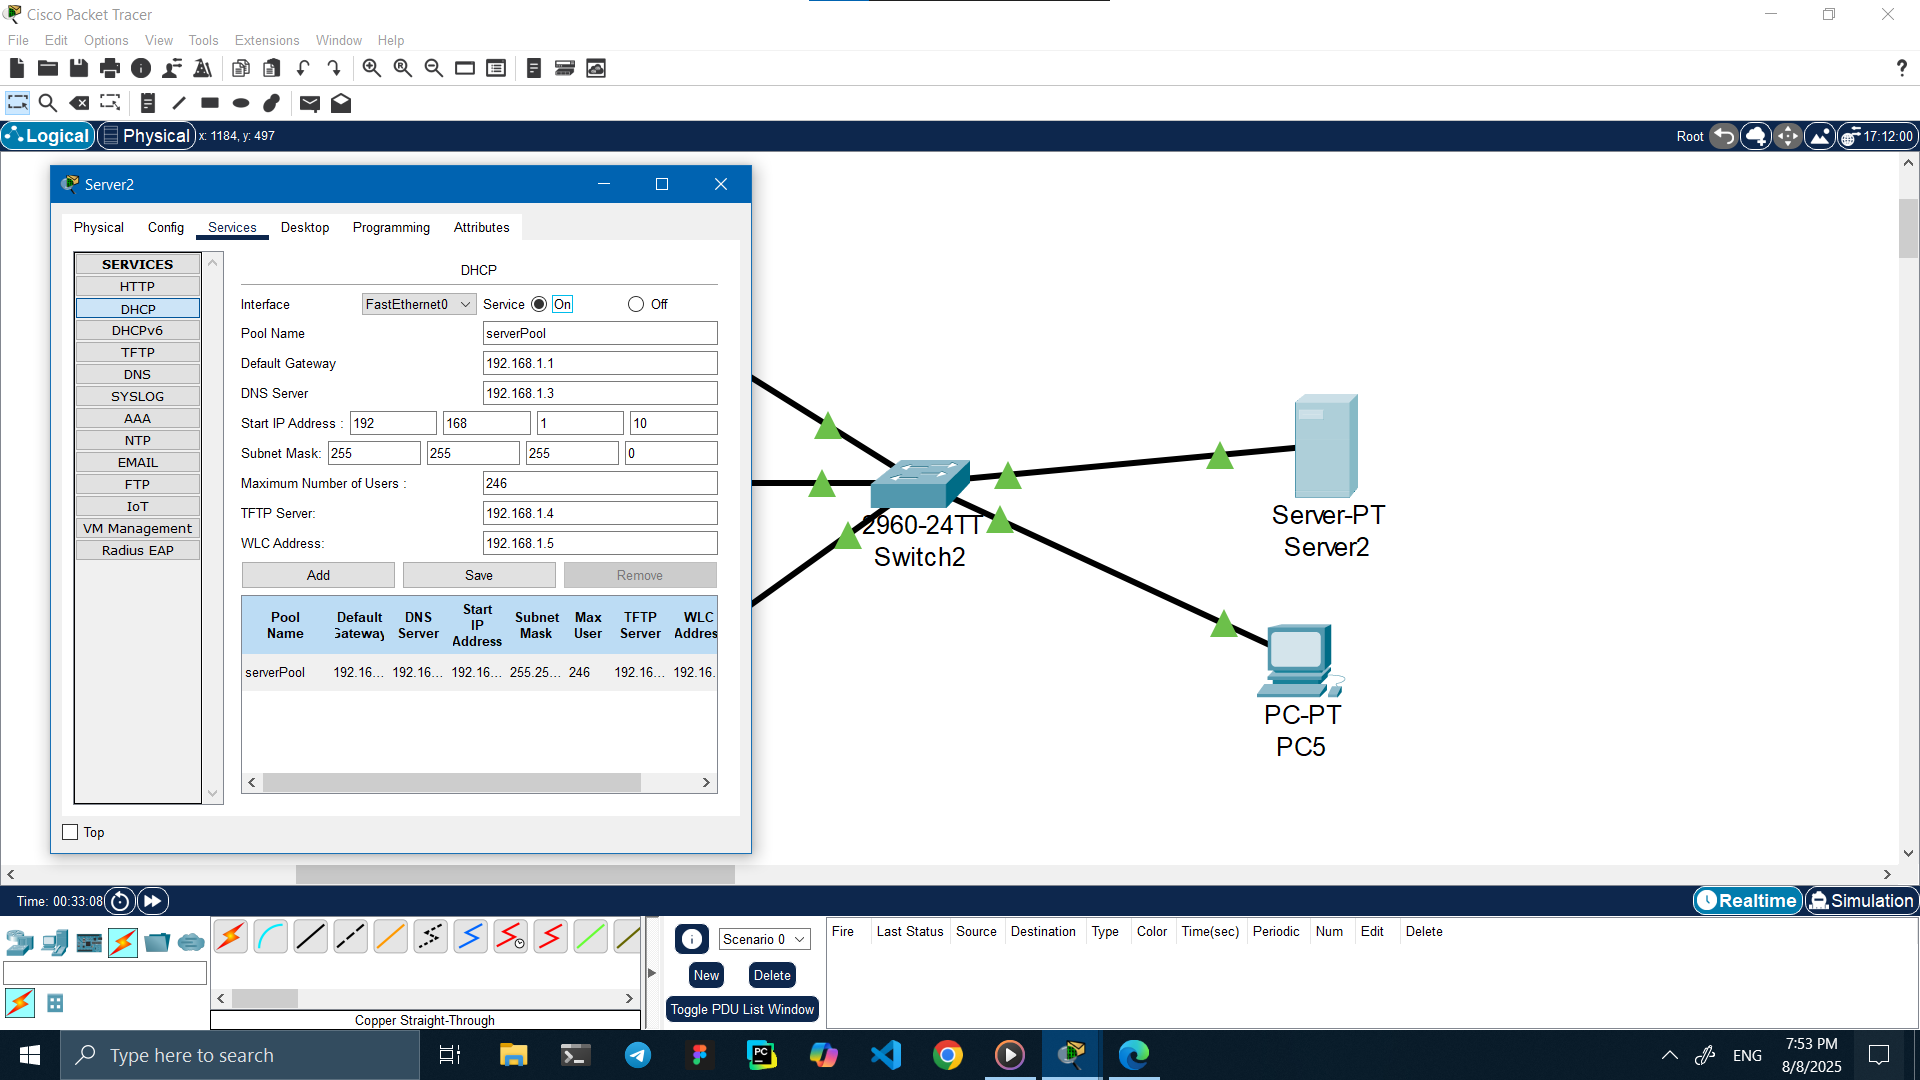
\includegraphics[width=\textwidth]{resources/scenario1-6.png}
		\caption{تنظیم سرویس \textenglish{DHCP} روی سرور و ایجاد \textenglish{pool} مناسب}
		\label{1:6}
	\end{figure}
	\begin{figure}[H]
		\centering
		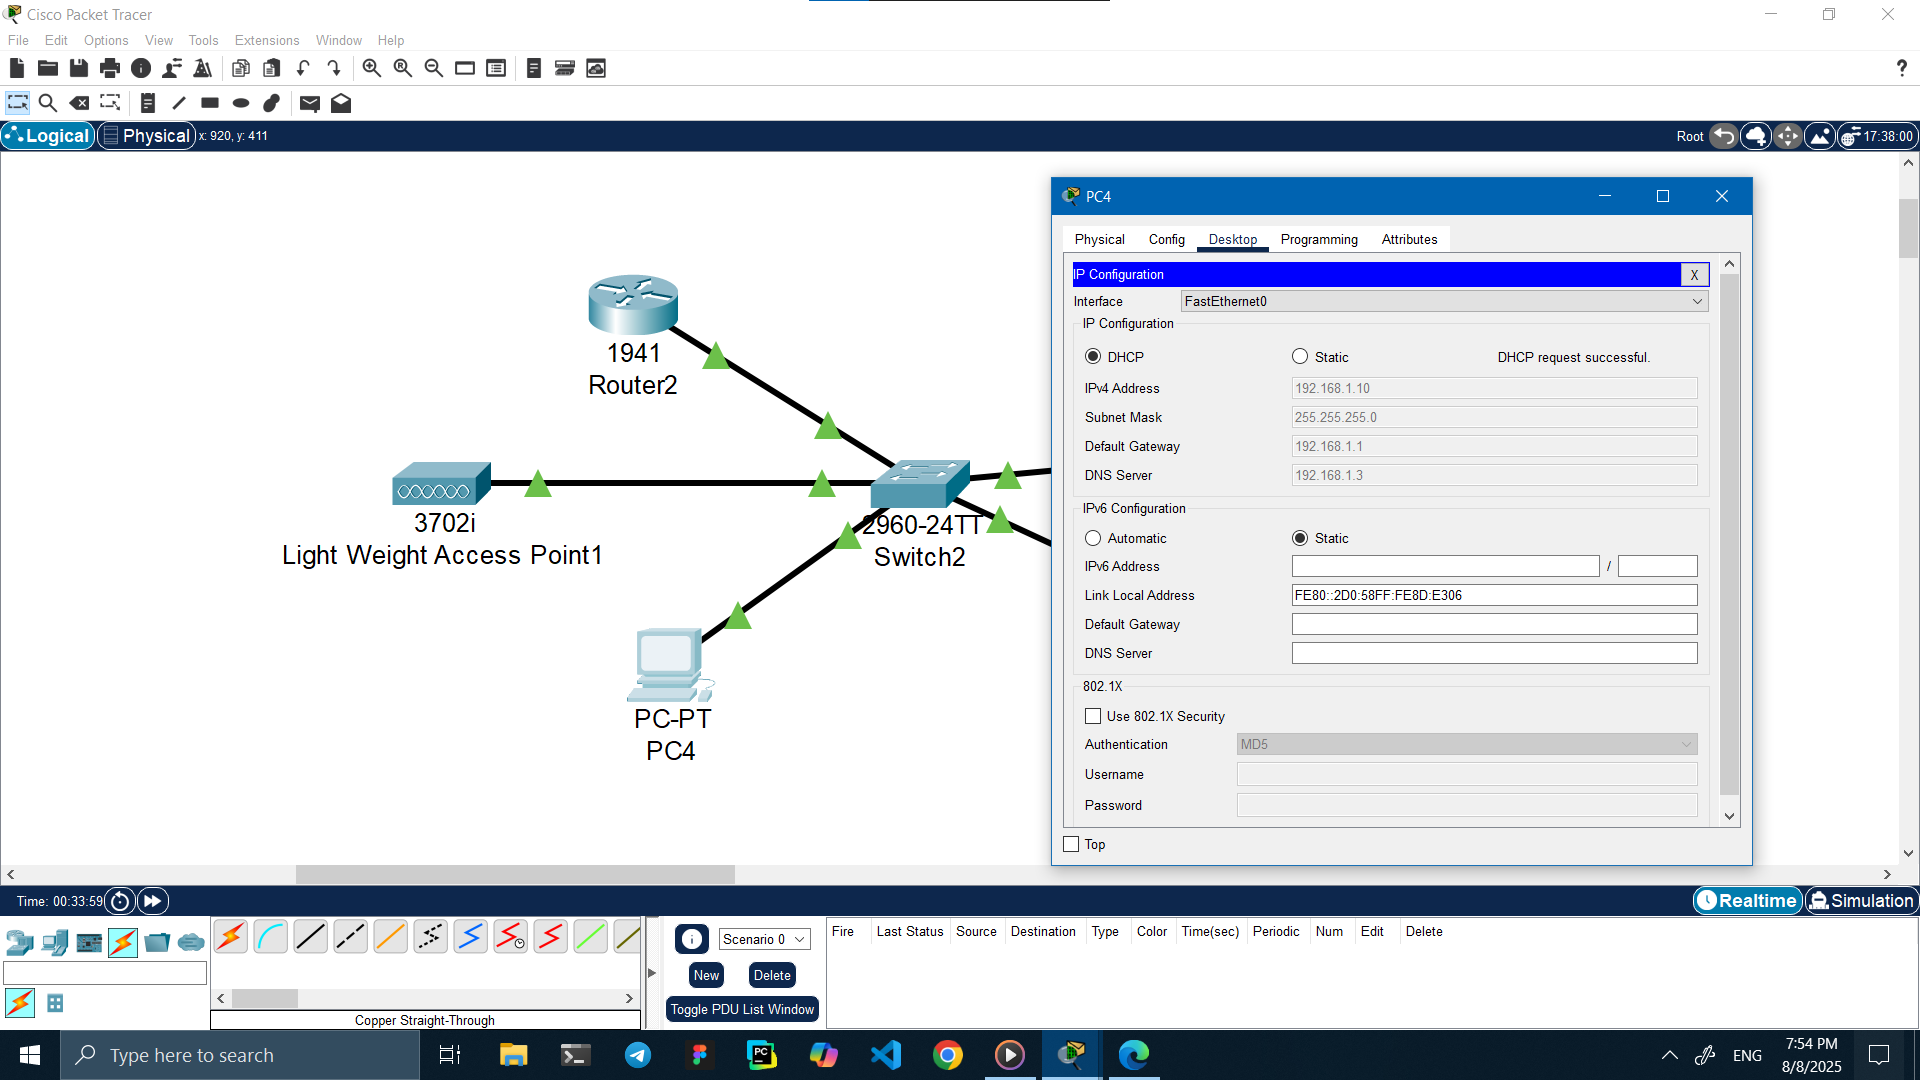
\includegraphics[width=\textwidth]{resources/scenario1-7.png}
		\caption{تنظیم \textenglish{PC} روی \textenglish{DHCP} برای دریافت \textenglish{ip} و مشاهده موفقیت‌آمیز بودن تخصیص}
		\label{1:7}
	\end{figure}
	\begin{figure}[H]
		\centering
		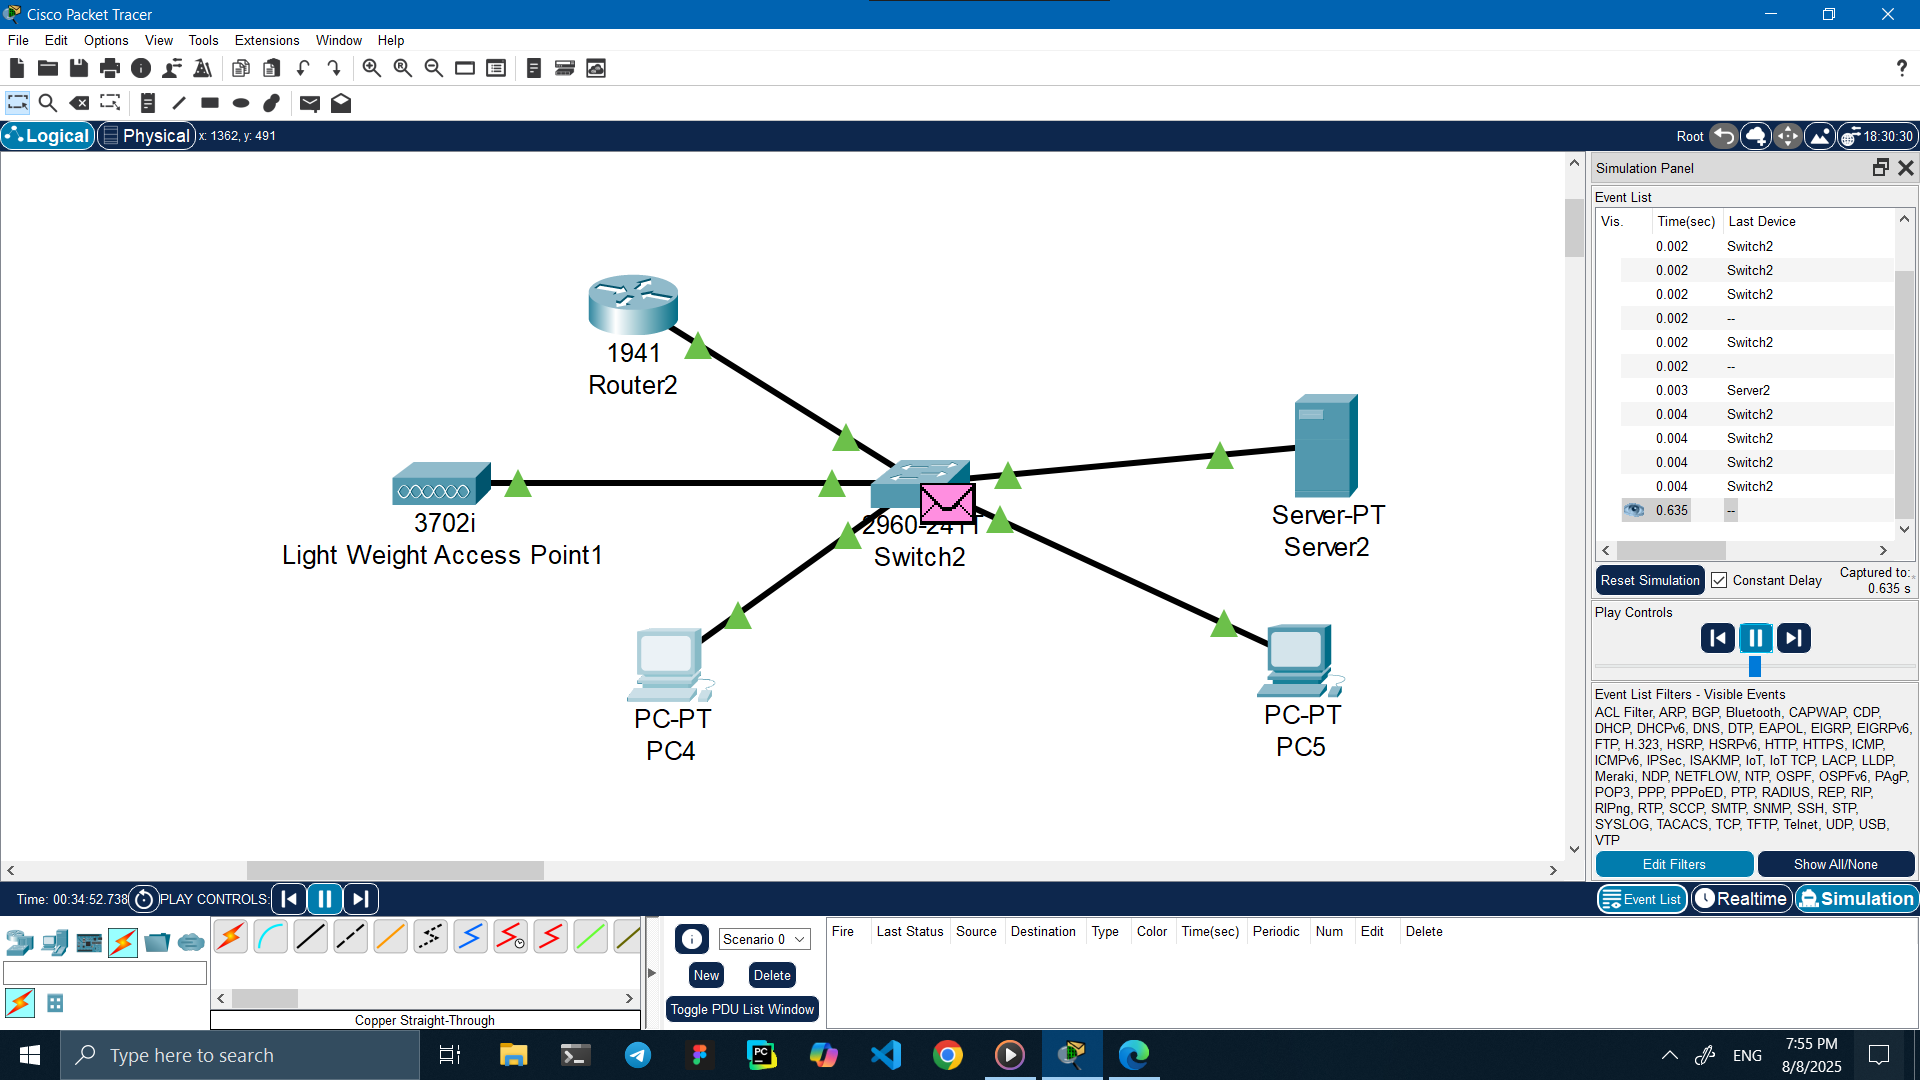
\includegraphics[width=\textwidth]{resources/scenario1-8.png}
		\caption{فرآیند شکل \ref{1:7} ولی در حالت \textenglish{simulation} و مشاهده حرکت بسته‌ها تا تخصیص آدرس}
		\label{1:8}
	\end{figure}
	\begin{figure}[H]
		\centering
		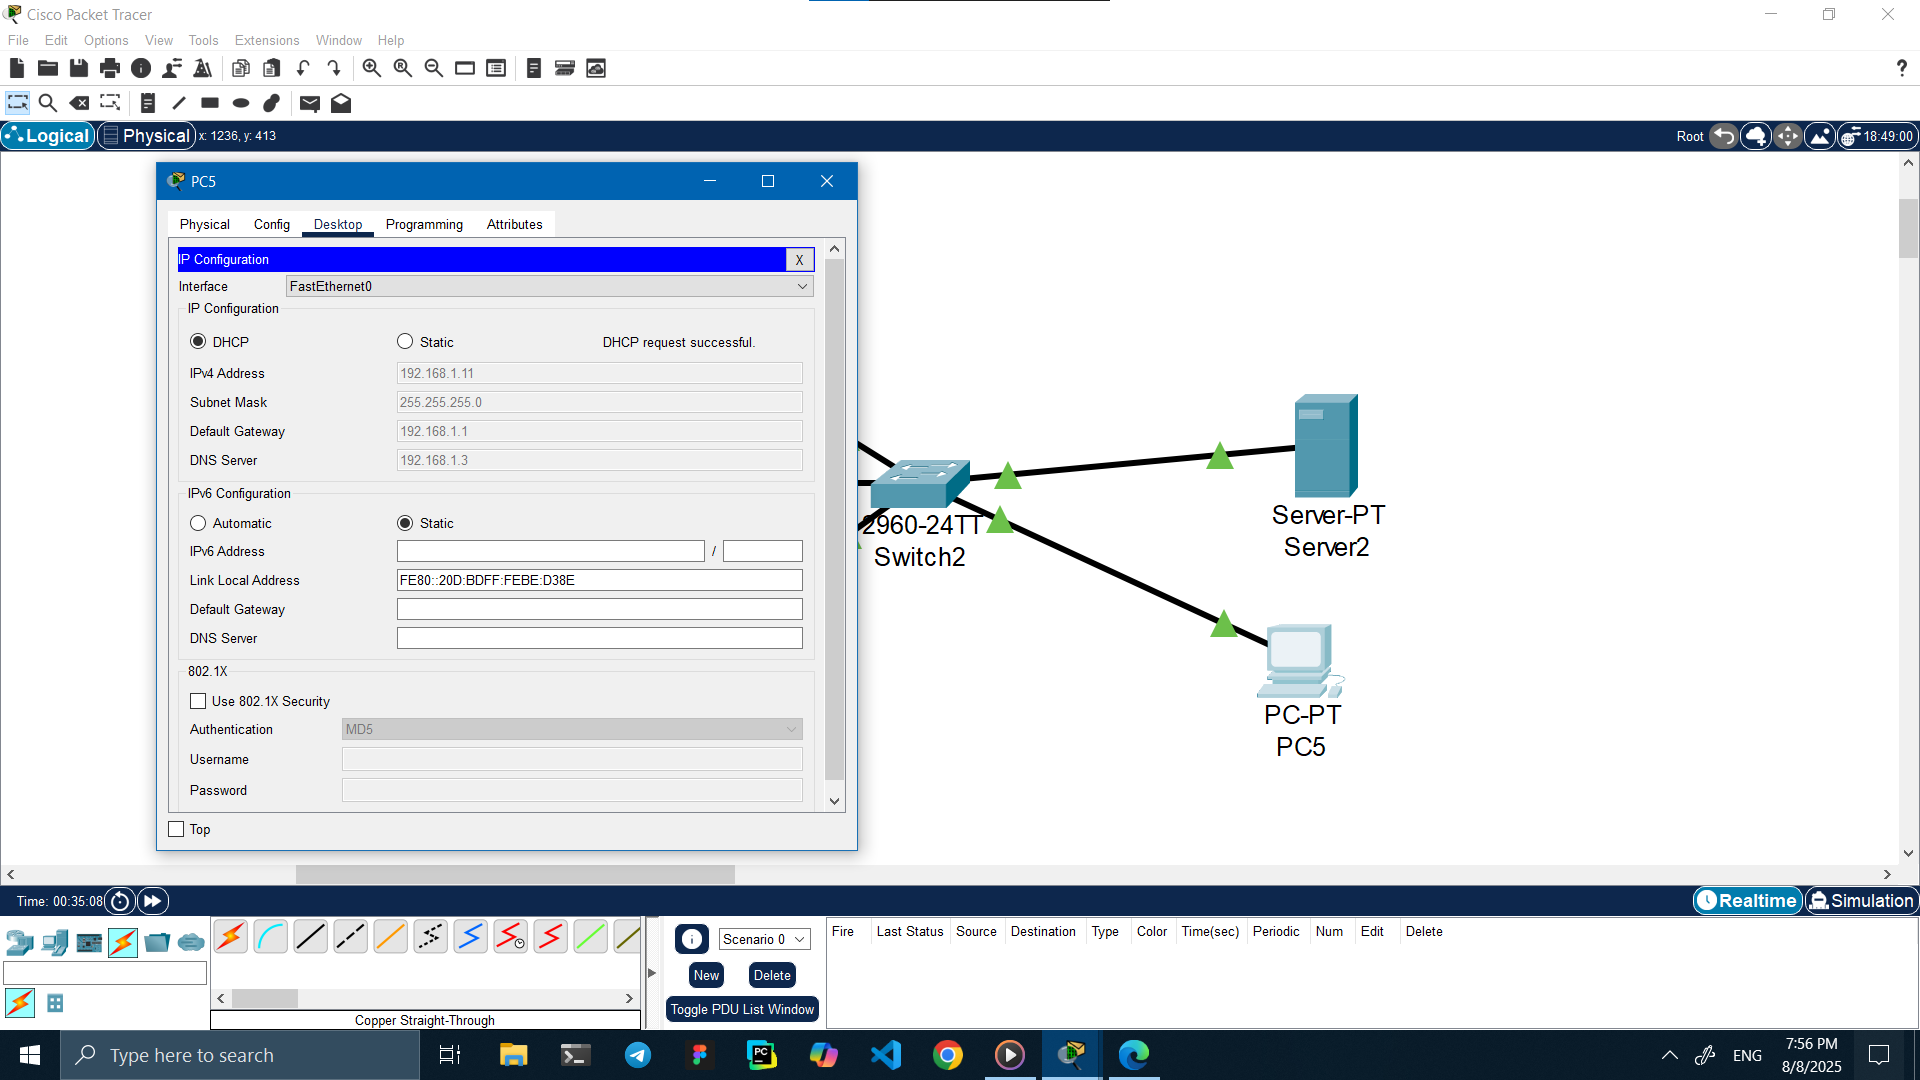
\includegraphics[width=\textwidth]{resources/scenario1-9.png}
		\caption{مراحل مشابهٔ شکل \ref{1:7} برای \textenglish{PC} دیگر در شبکه}
		\label{1:9}
	\end{figure}
	\newpage
	\section{سناریو ۲}
	\begin{figure}[H]
		\centering
		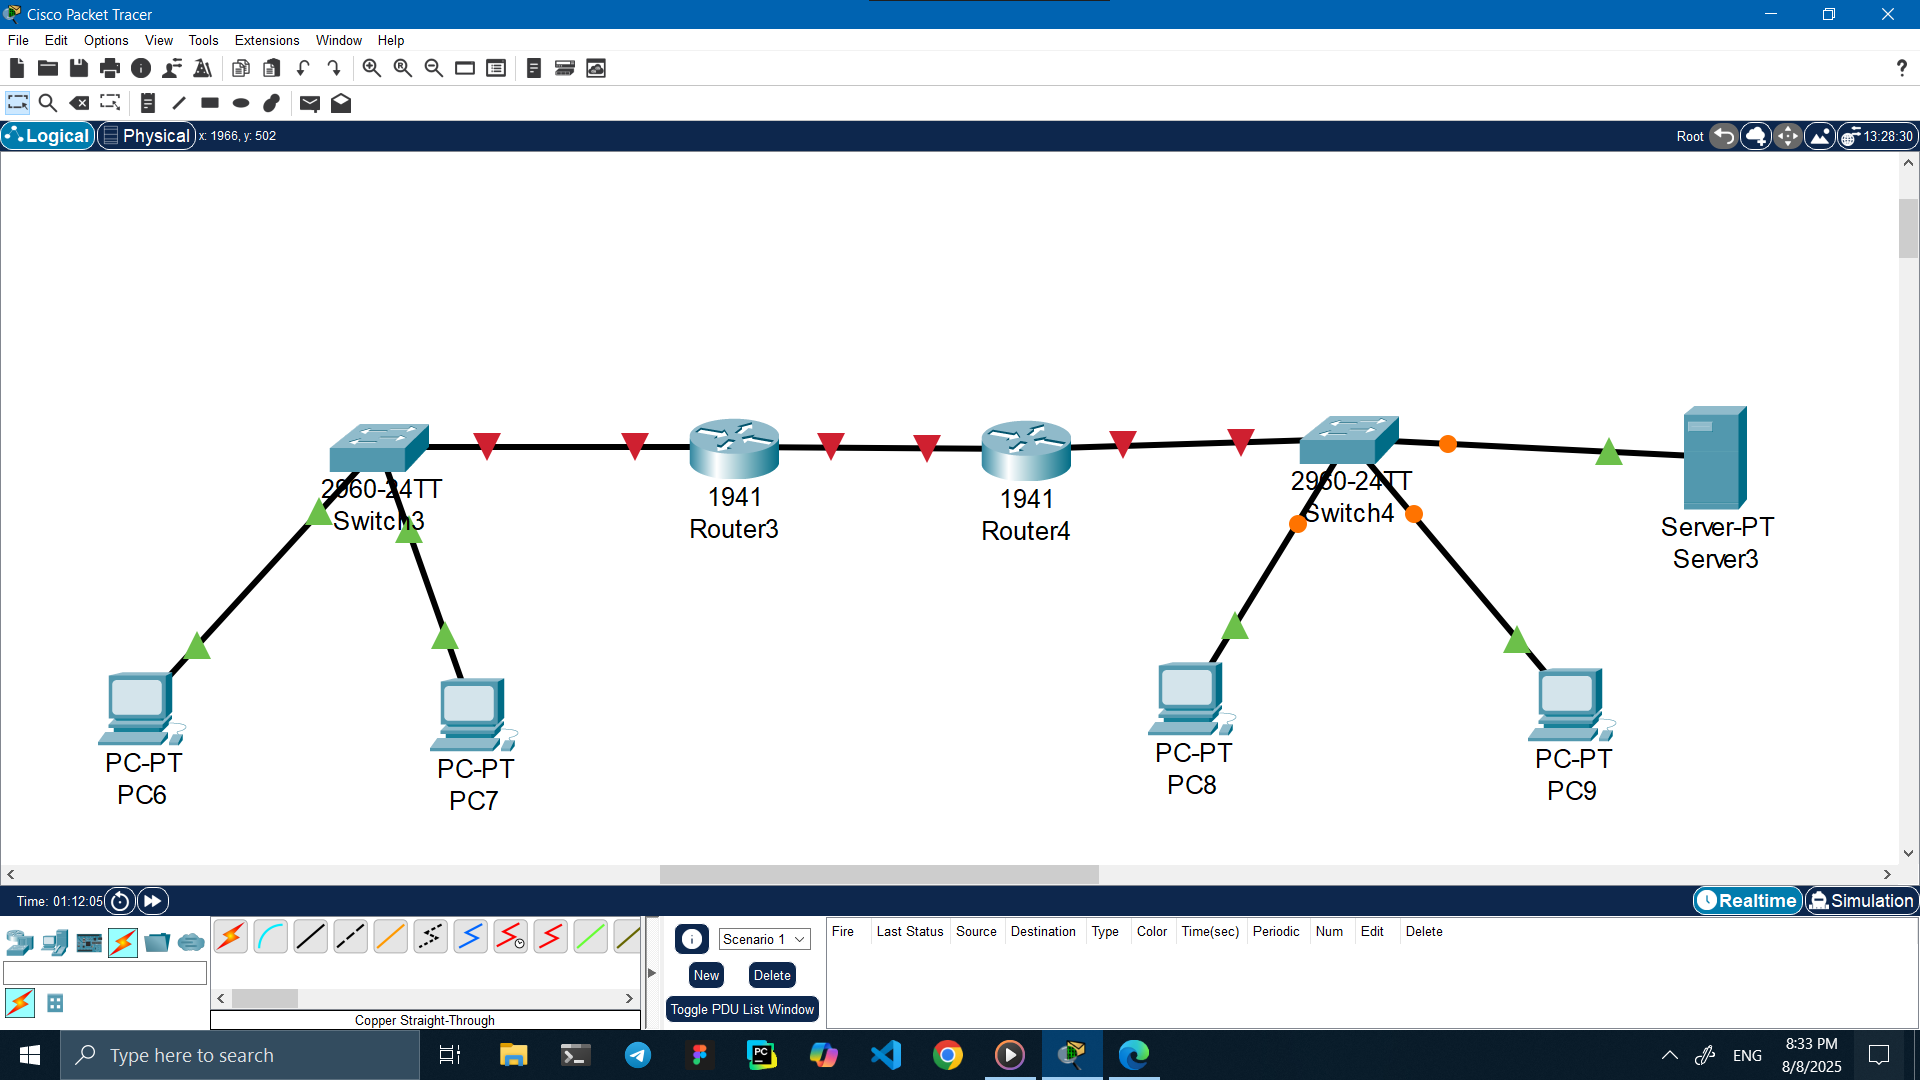
\includegraphics[width=\textwidth]{resources/scenario2-1.png}
		\caption{اضافه کردن دستگاه‌ها و اتصالات سناریو ۲}
		\label{2:1}
	\end{figure}
	\begin{figure}[H]
		\centering
		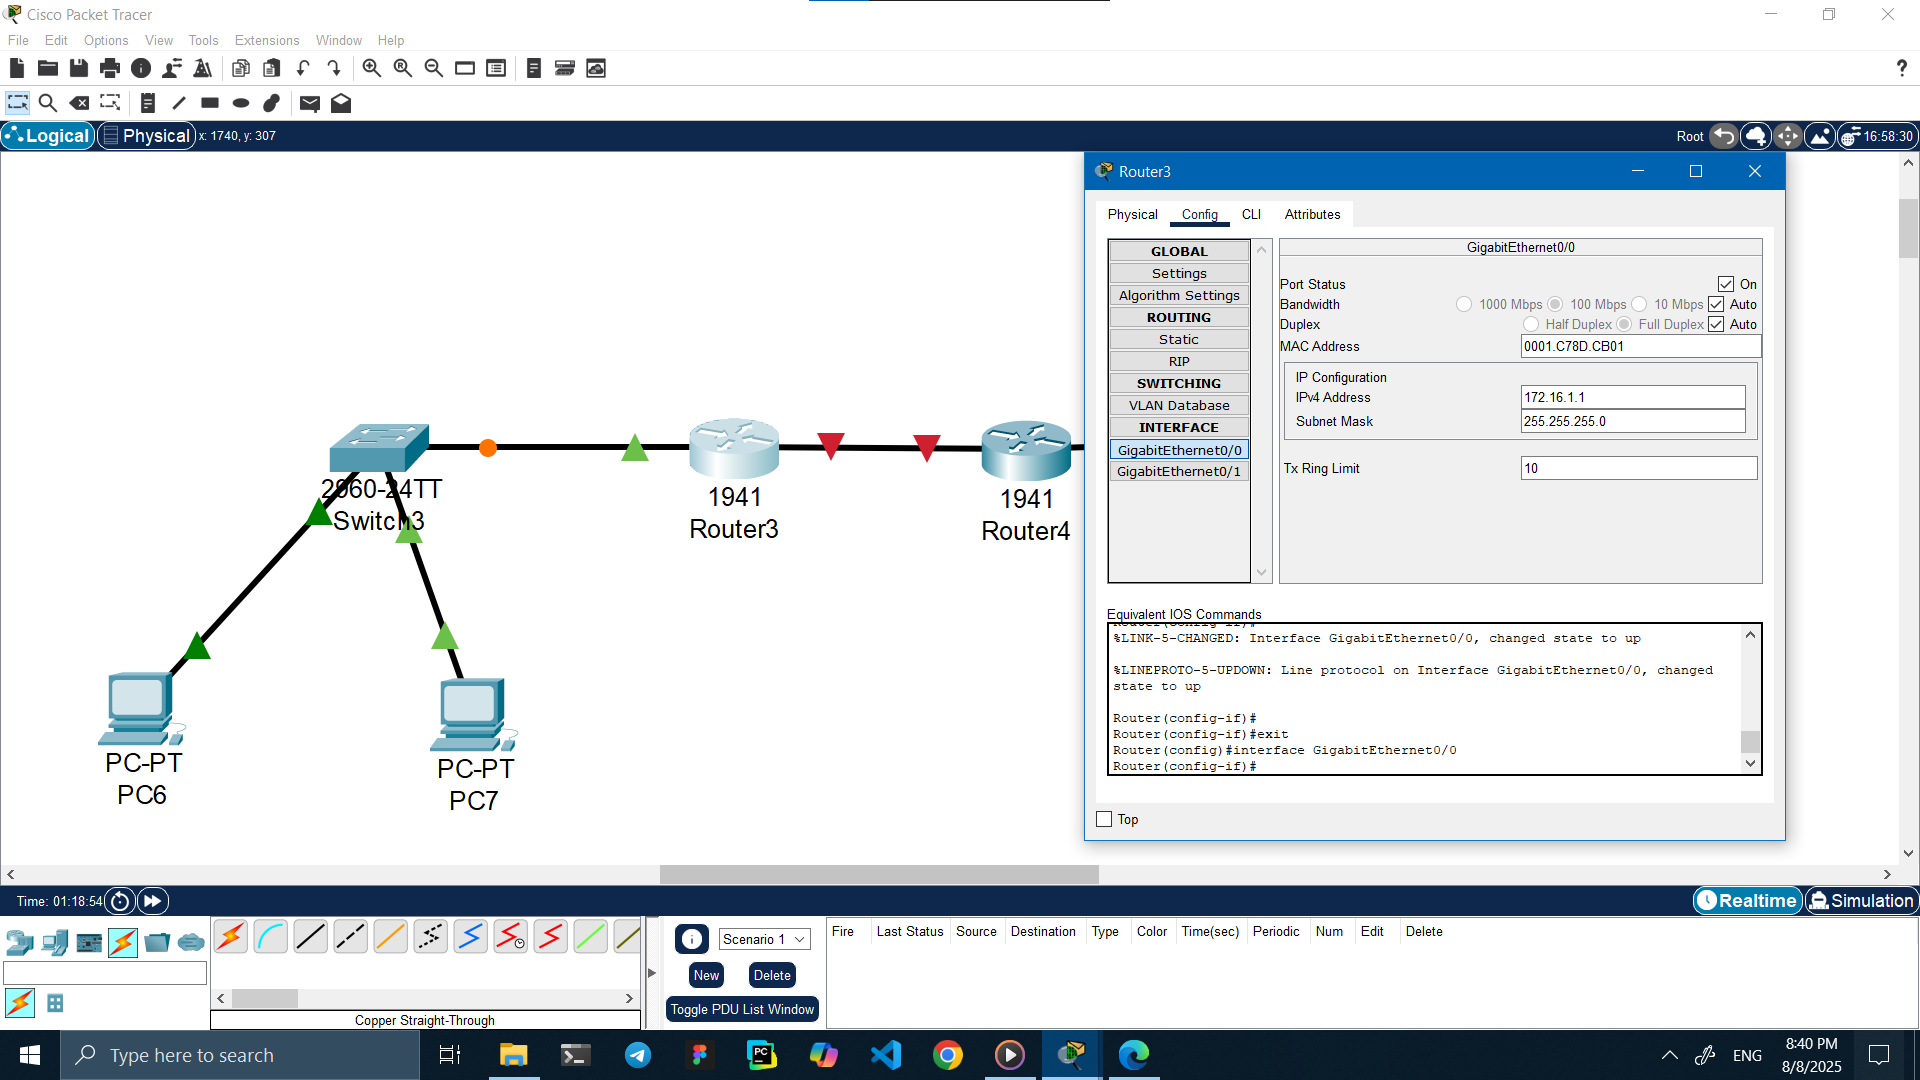
\includegraphics[width=\textwidth]{resources/scenario2-2.png}
		\caption{تنظیم \textenglish{ip} برای واسط \textenglish{Gig0/0} در \textenglish{Router} سمت چپ}
		\label{2:2}
	\end{figure}
	\begin{figure}[H]
		\centering
		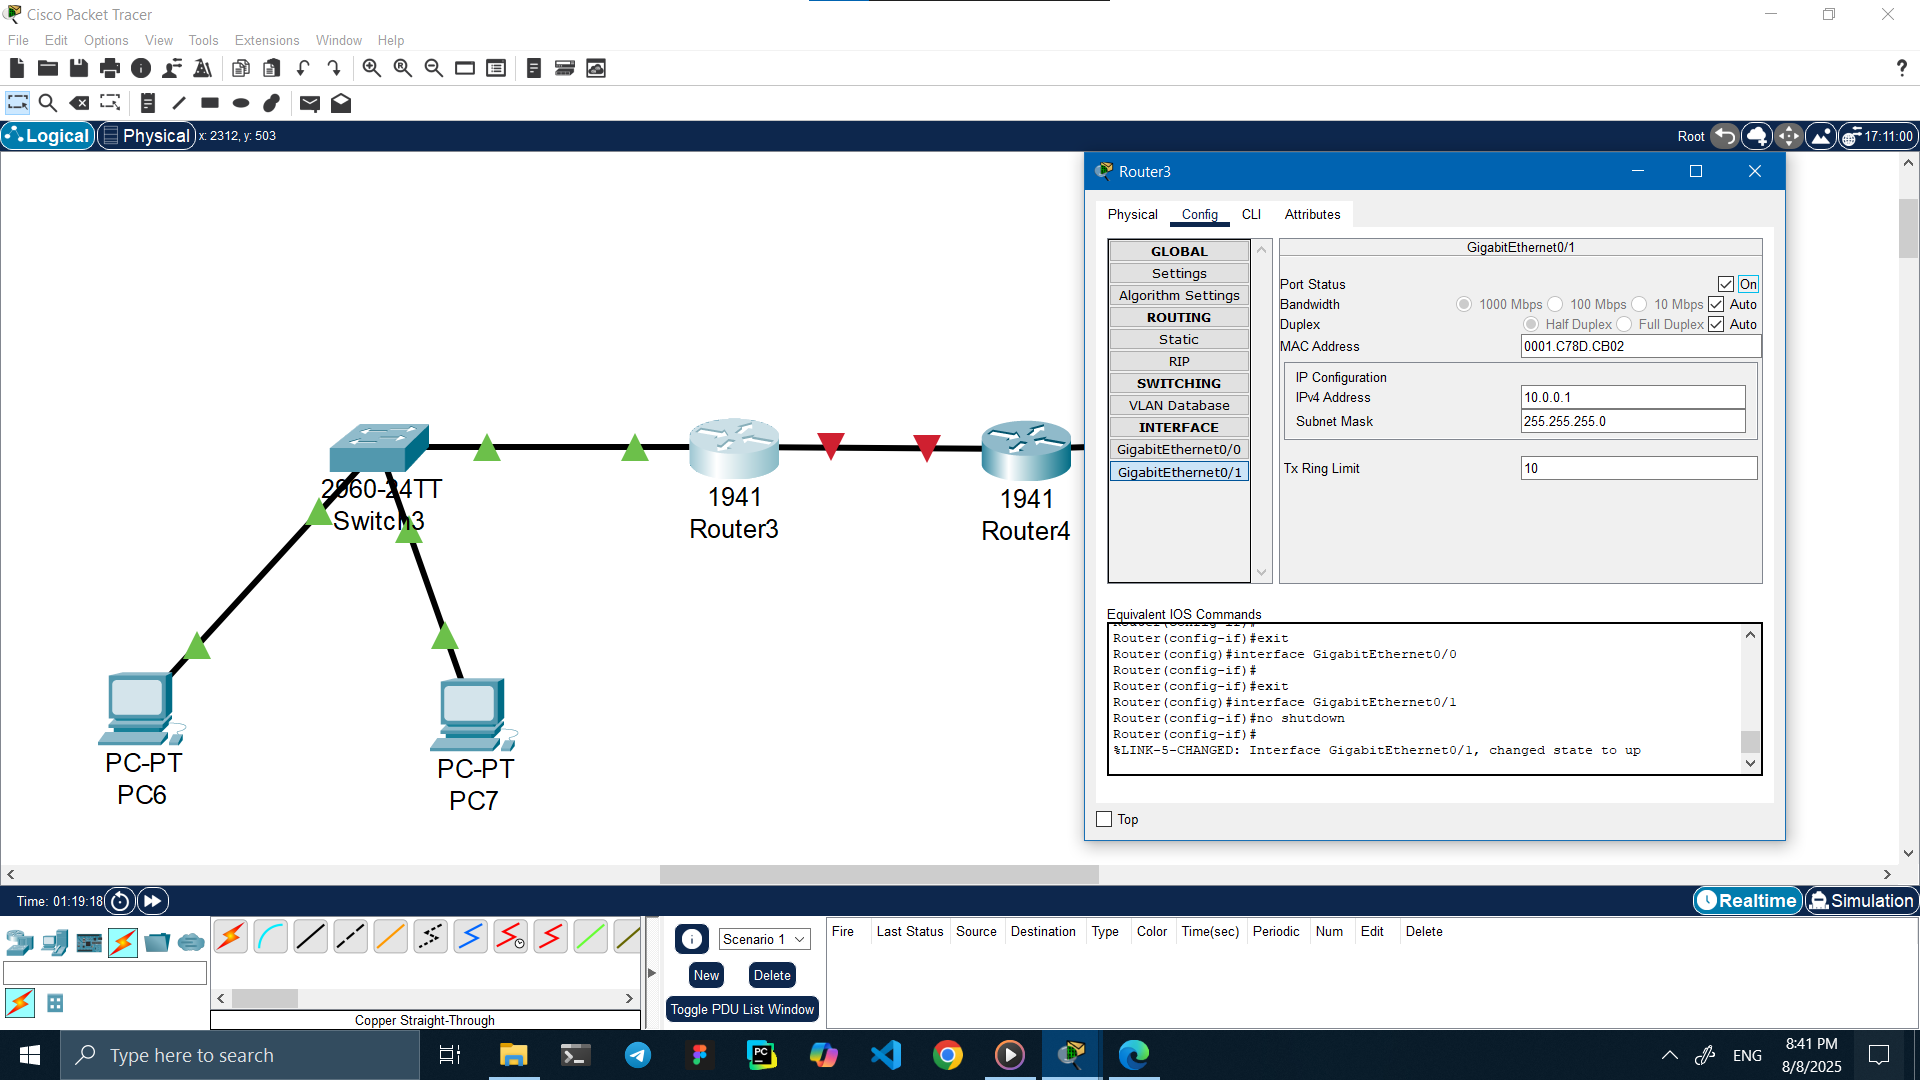
\includegraphics[width=\textwidth]{resources/scenario2-3.png}
		\caption{تنظیم \textenglish{ip} برای واسط \textenglish{Gig0/1} در \textenglish{Router} سمت چپ}
		\label{2:3}
	\end{figure}
	\begin{figure}[H]
		\centering
		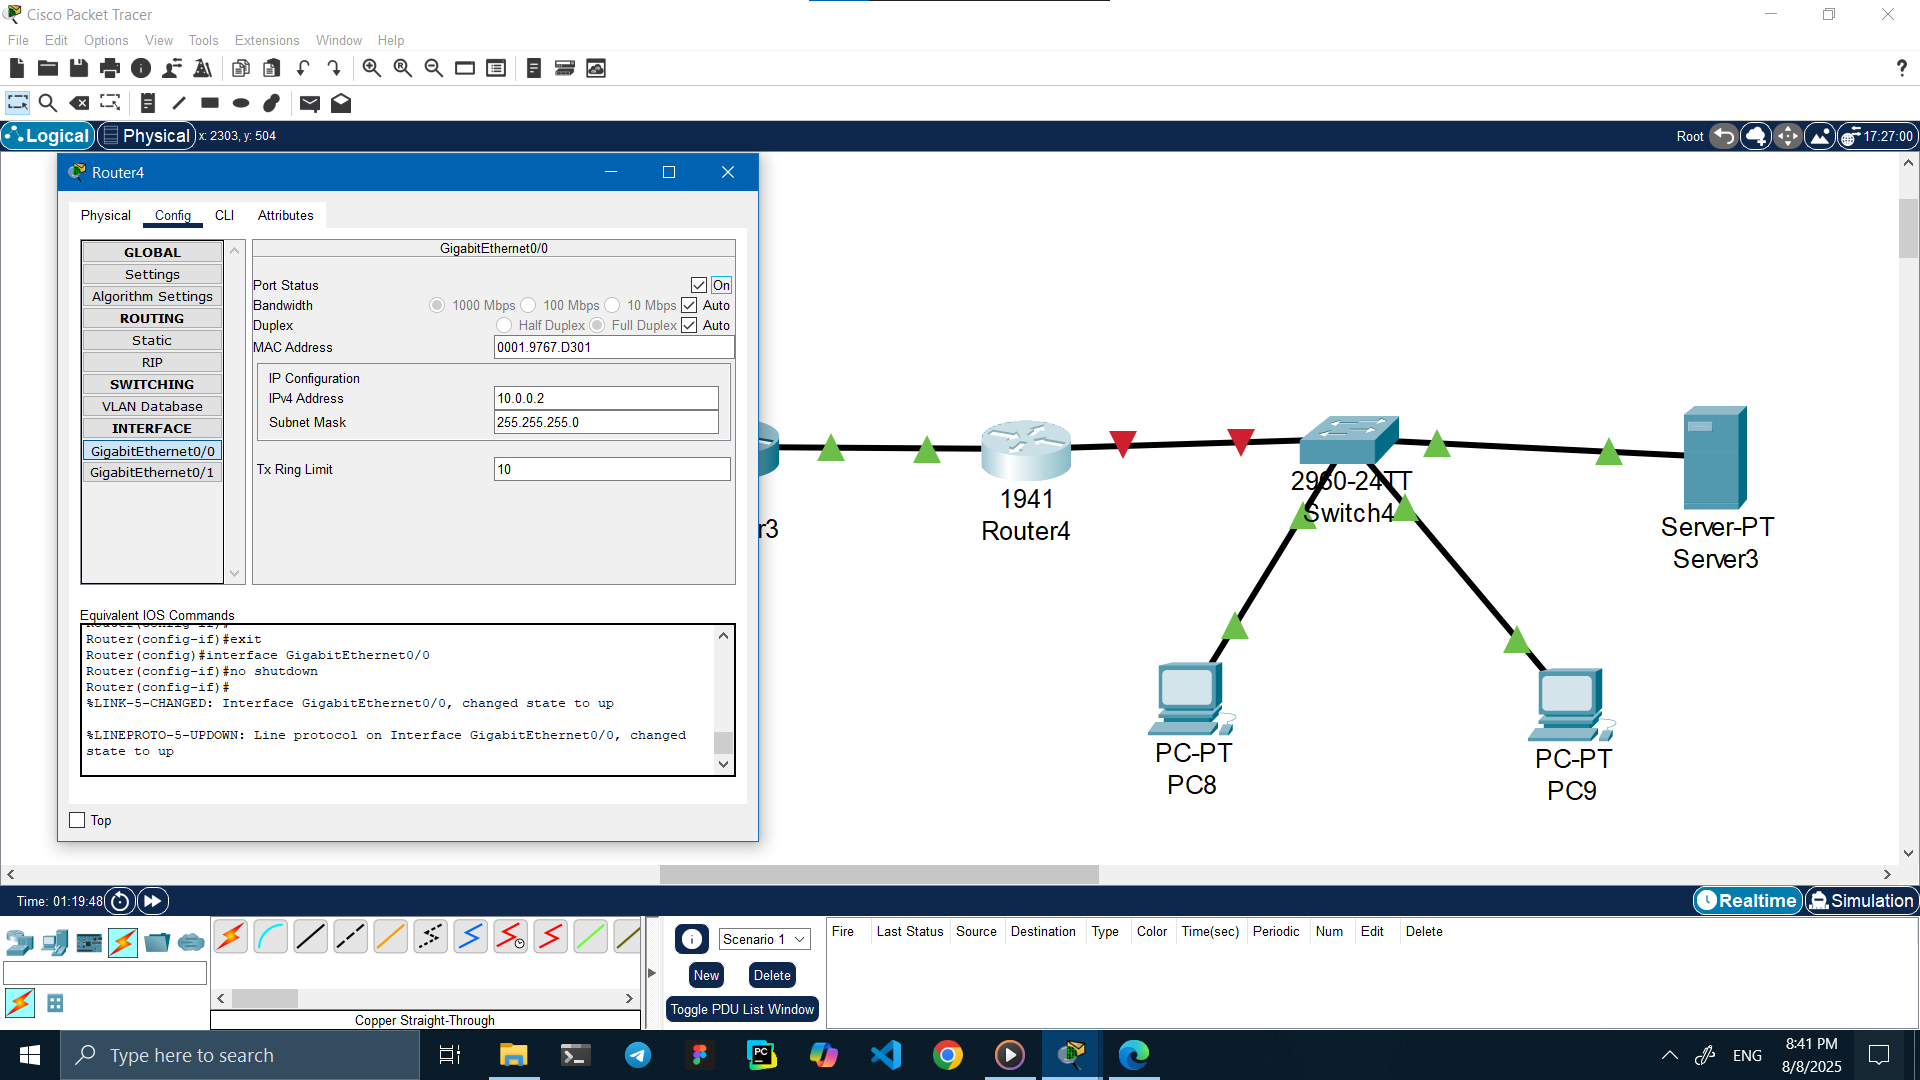
\includegraphics[width=\textwidth]{resources/scenario2-4.png}
		\caption{تنظیم \textenglish{ip} برای واسط \textenglish{Gig0/0} در \textenglish{Router} سمت راست}
		\label{2:4}
	\end{figure}
	\begin{figure}[H]
		\centering
		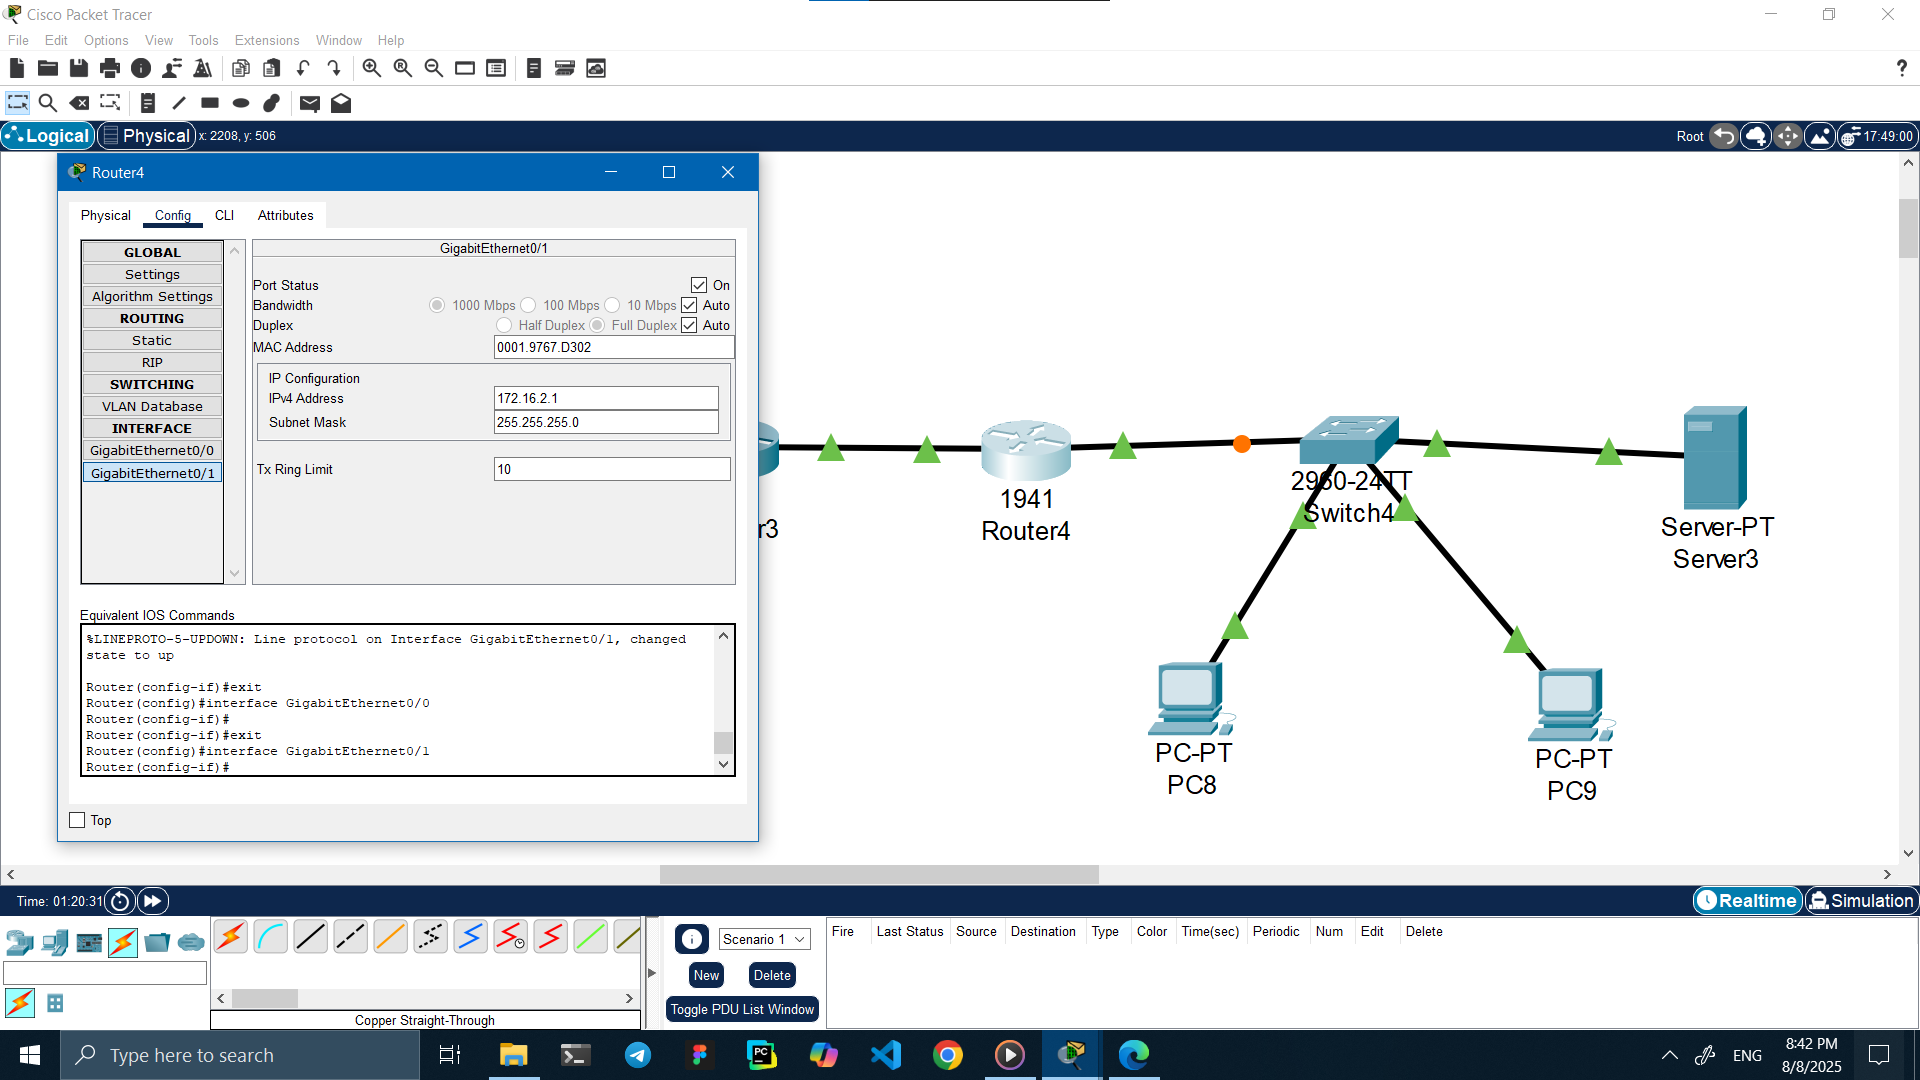
\includegraphics[width=\textwidth]{resources/scenario2-5.png}
		\caption{تنظیم \textenglish{ip} برای واسط \textenglish{Gig0/1} در \textenglish{Router} سمت راست}
		\label{2:5}
	\end{figure}
	\begin{figure}[H]
		\centering
		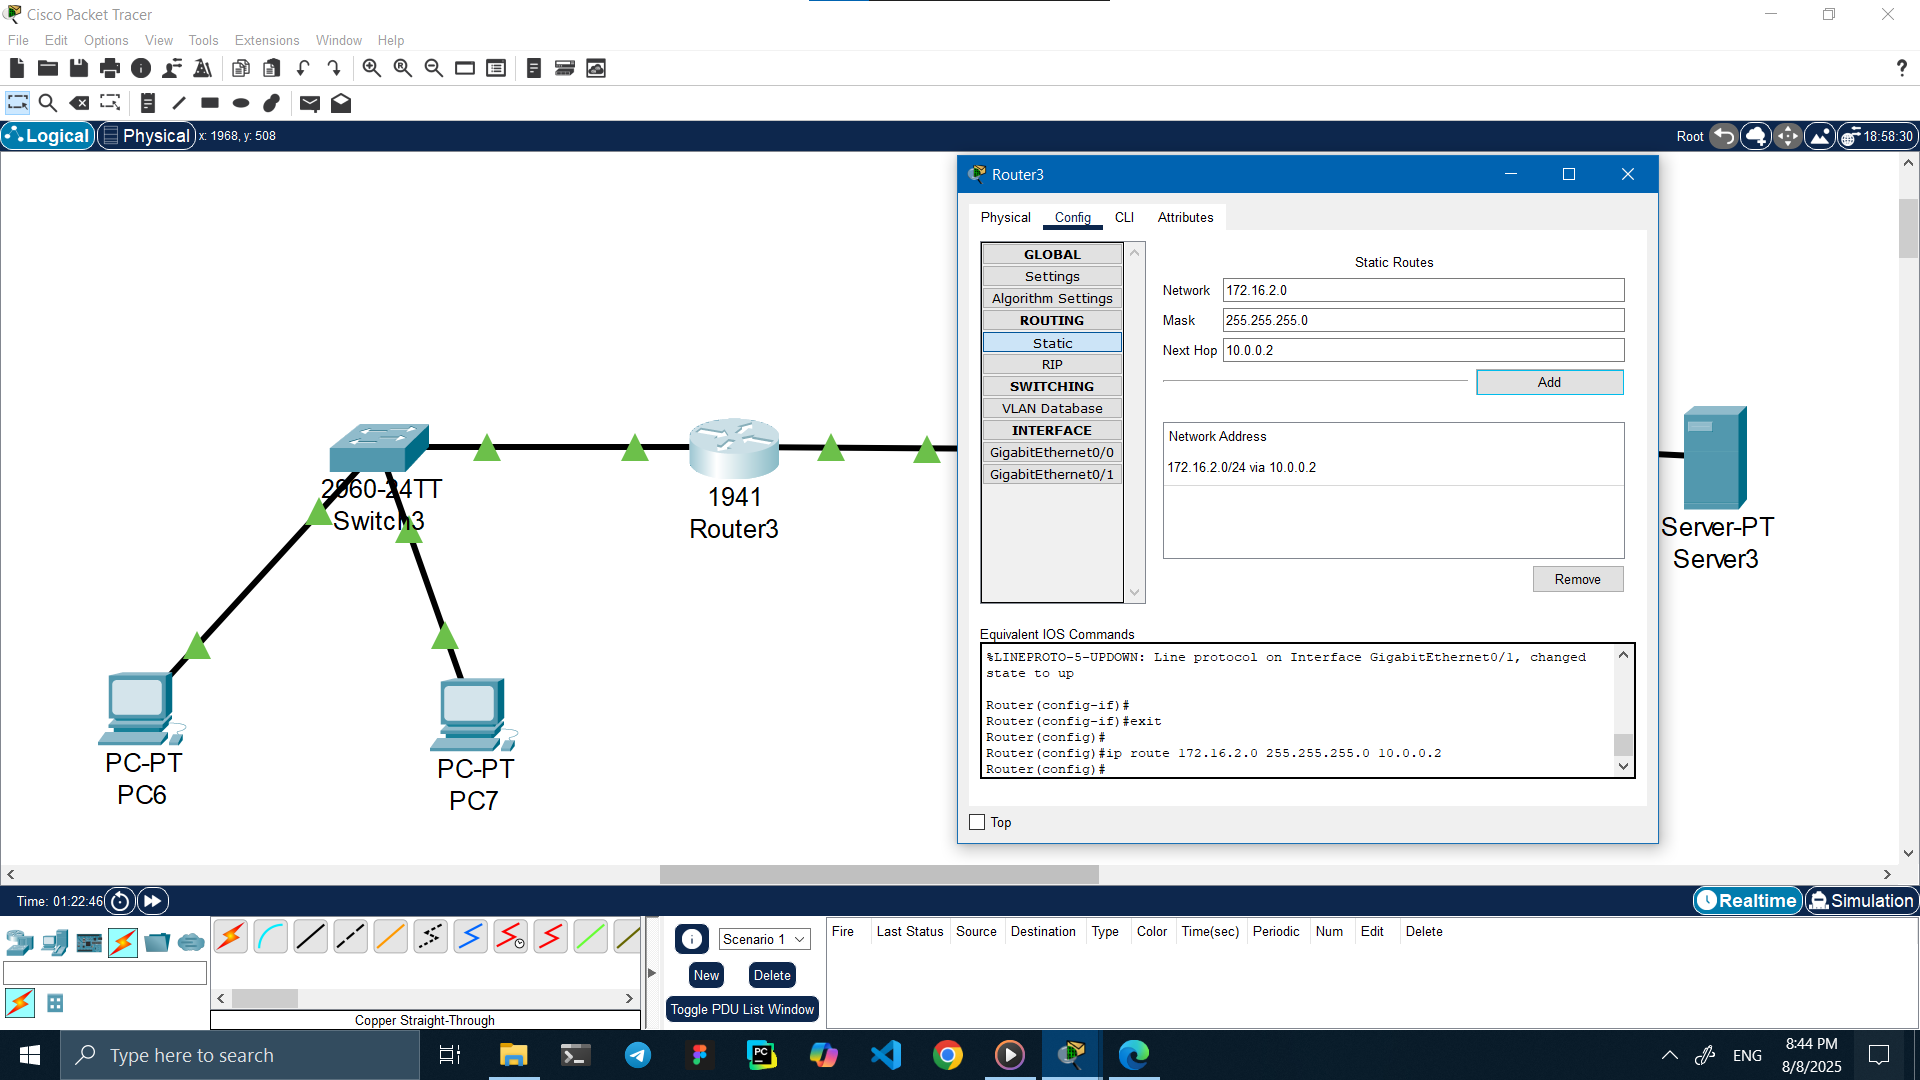
\includegraphics[width=\textwidth]{resources/scenario2-6.png}
		\caption{تنظیم \textenglish{Routing} به شبکهٔ مجاور برای \textenglish{Router} سمت چپ}
		\label{2:6}
	\end{figure}
	\begin{figure}[H]
		\centering
		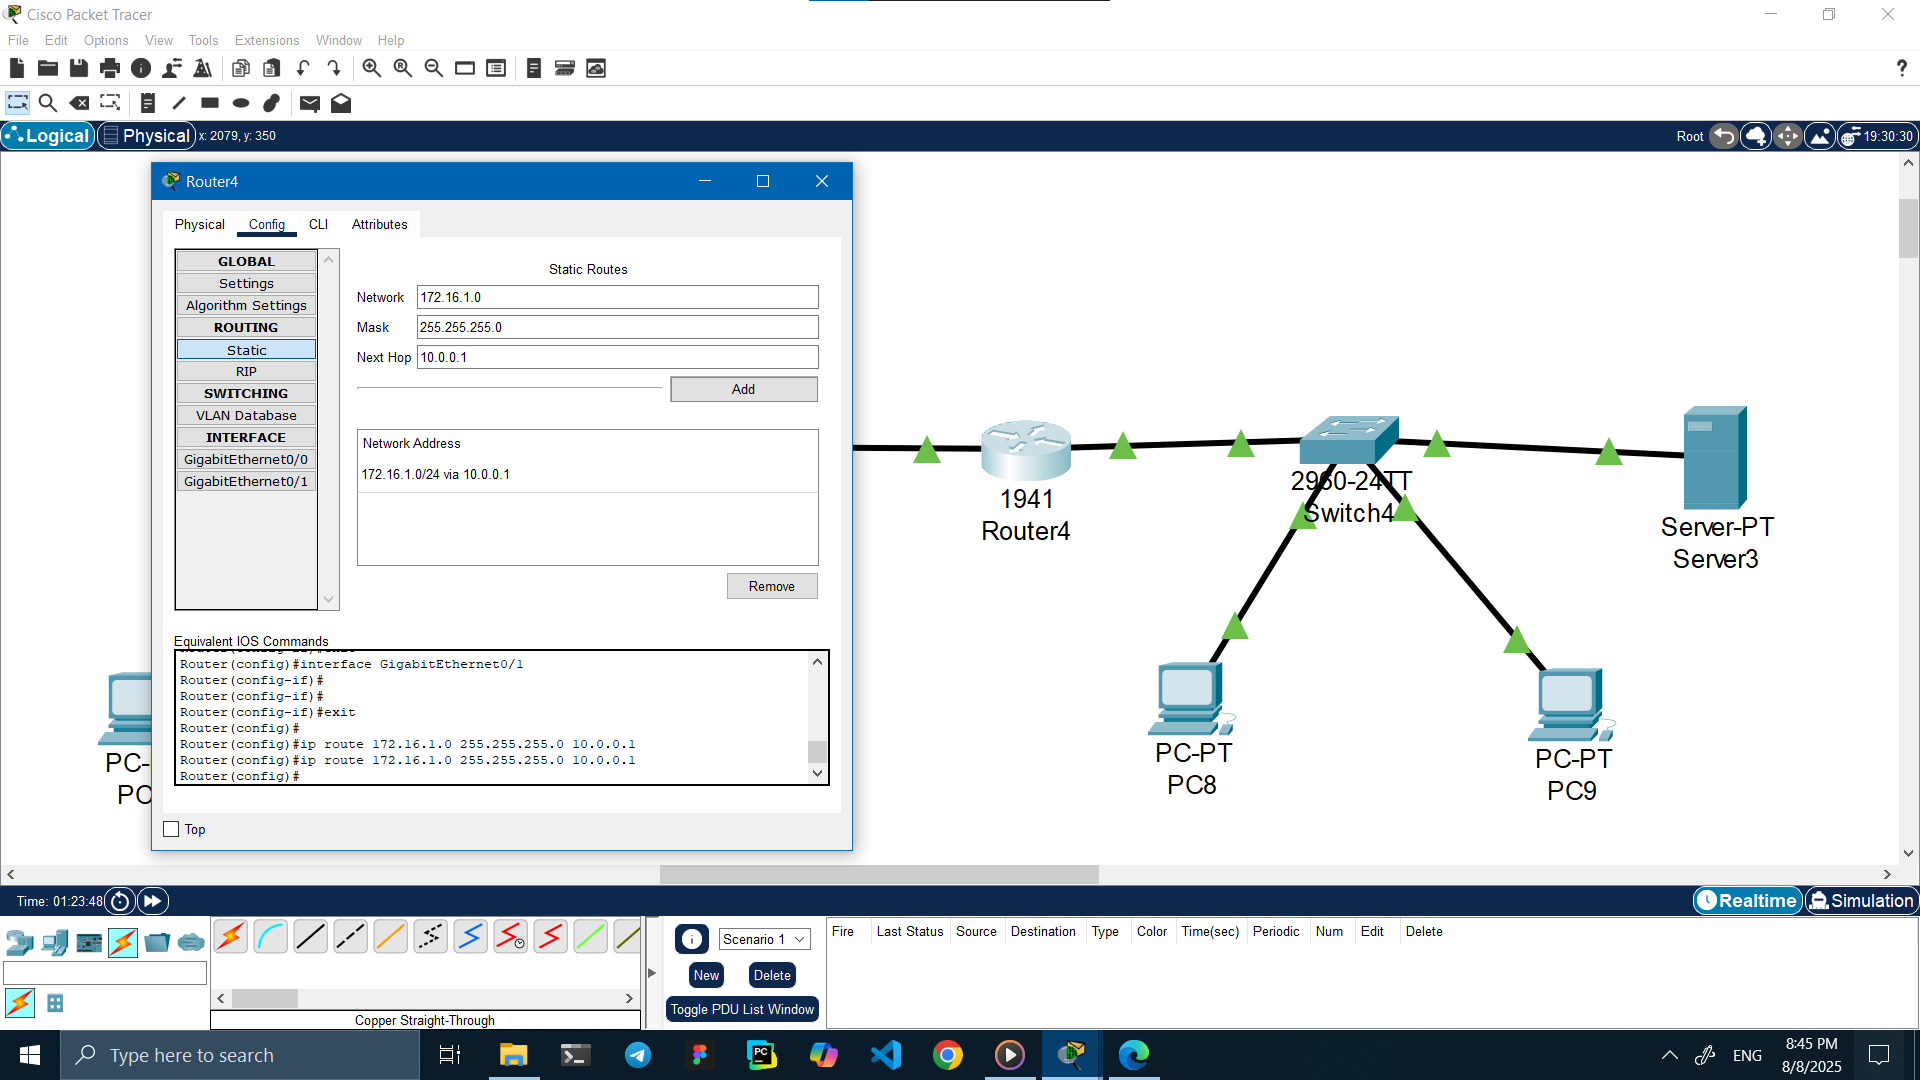
\includegraphics[width=\textwidth]{resources/scenario2-7.png}
		\caption{تنظیم \textenglish{Routing} به شبکهٔ مجاور برای \textenglish{Router} سمت راست}
		\label{2:7}
	\end{figure}
	\begin{figure}[H]
		\centering
		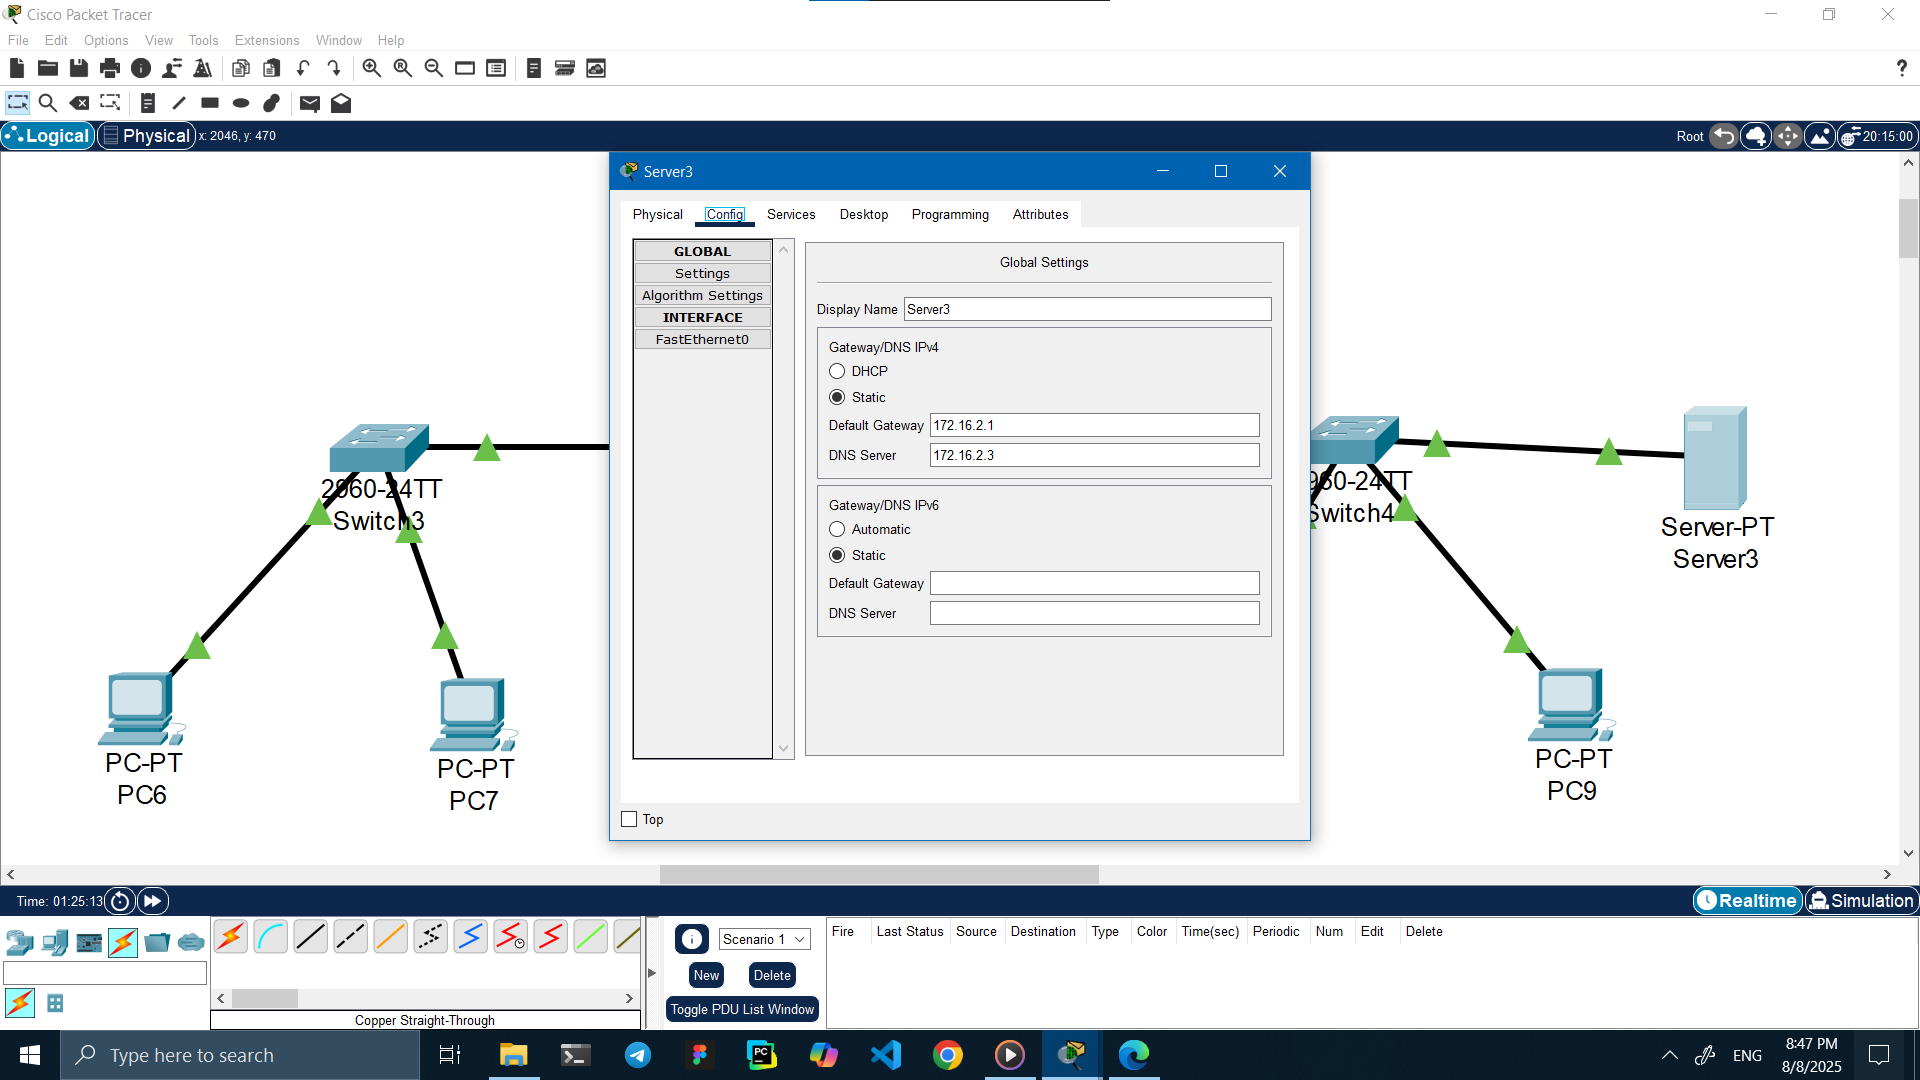
\includegraphics[width=\textwidth]{resources/scenario2-8.png}
		\caption{اضافه کردن \textenglish{Default Gateway} و \textenglish{DNS Server} در تنظیمات سرور}
		\label{2:8}
	\end{figure}
	\begin{figure}[H]
		\centering
		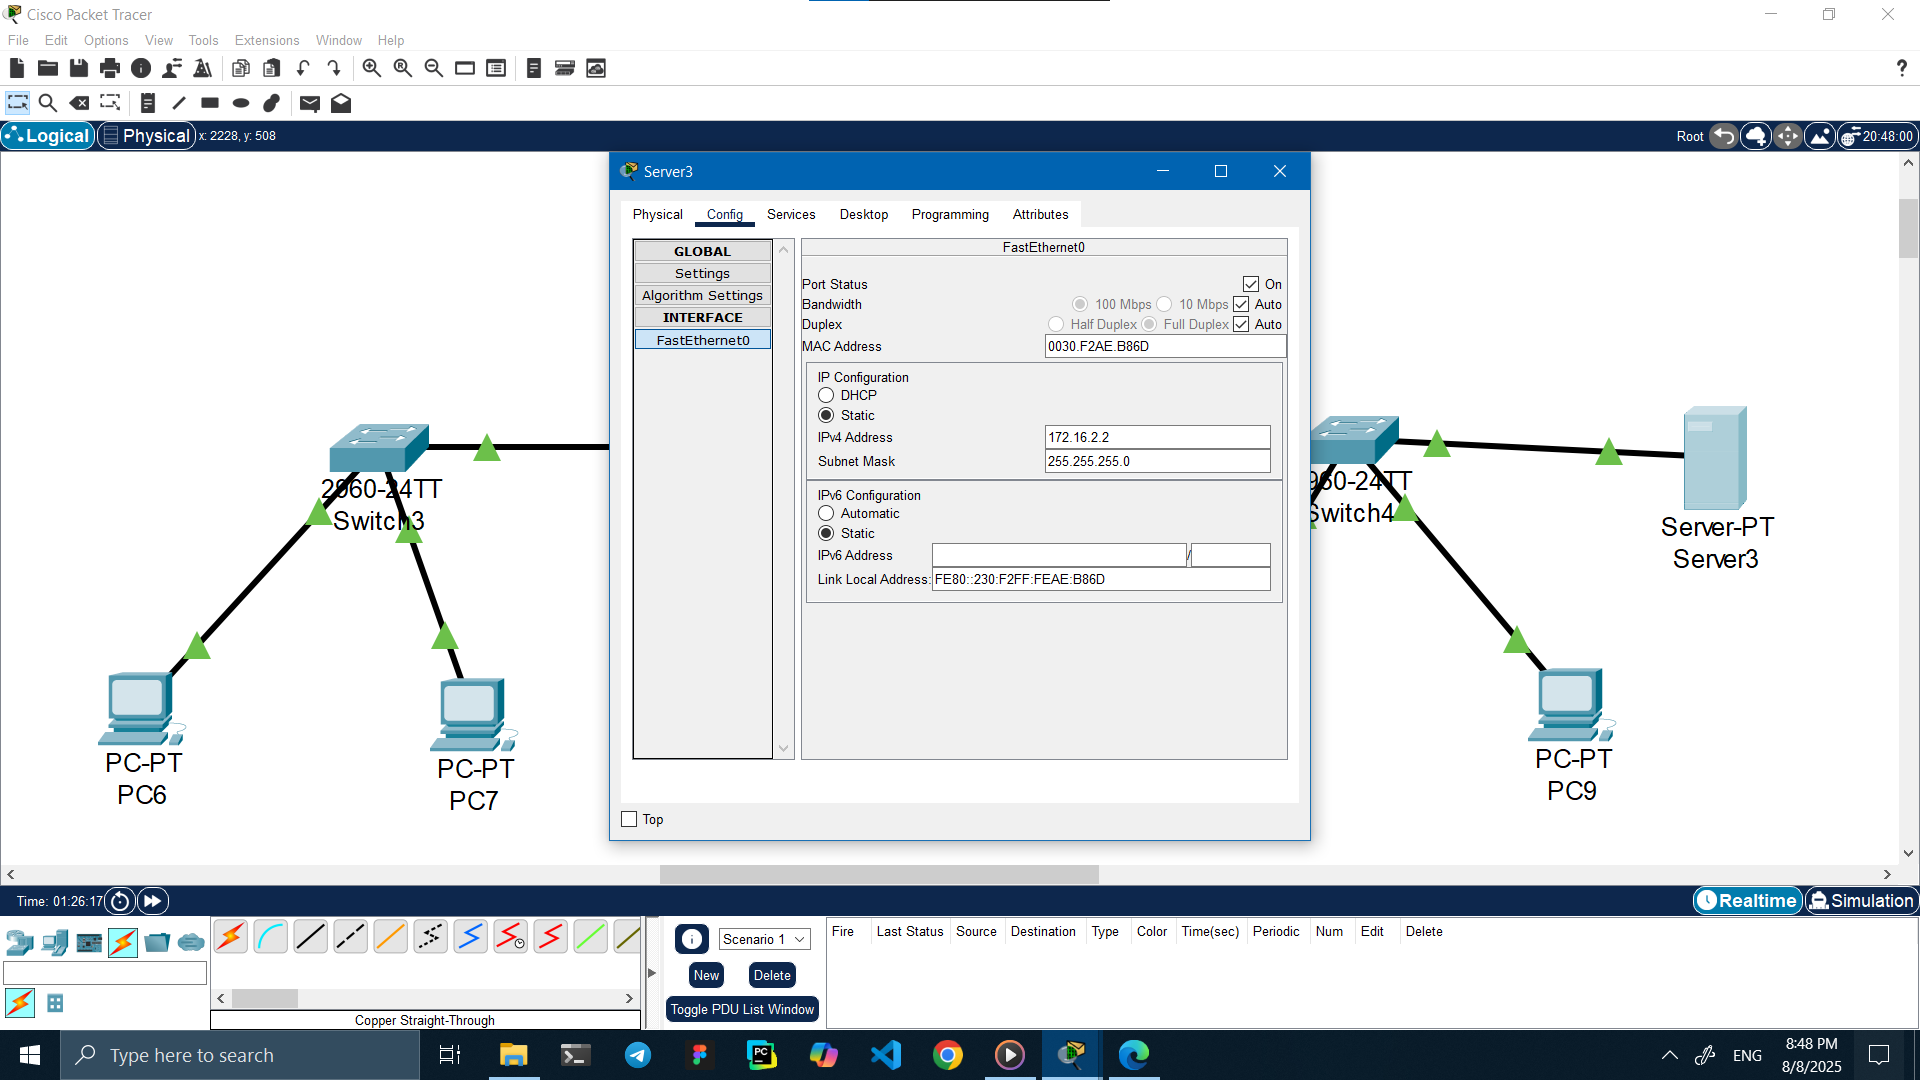
\includegraphics[width=\textwidth]{resources/scenario2-9.png}
		\caption{تنظیم آدرس \textenglish{ip} سرور و اطمینان از روشن بودن آن}
		\label{2:9}
	\end{figure}
	\begin{figure}[H]
		\centering
		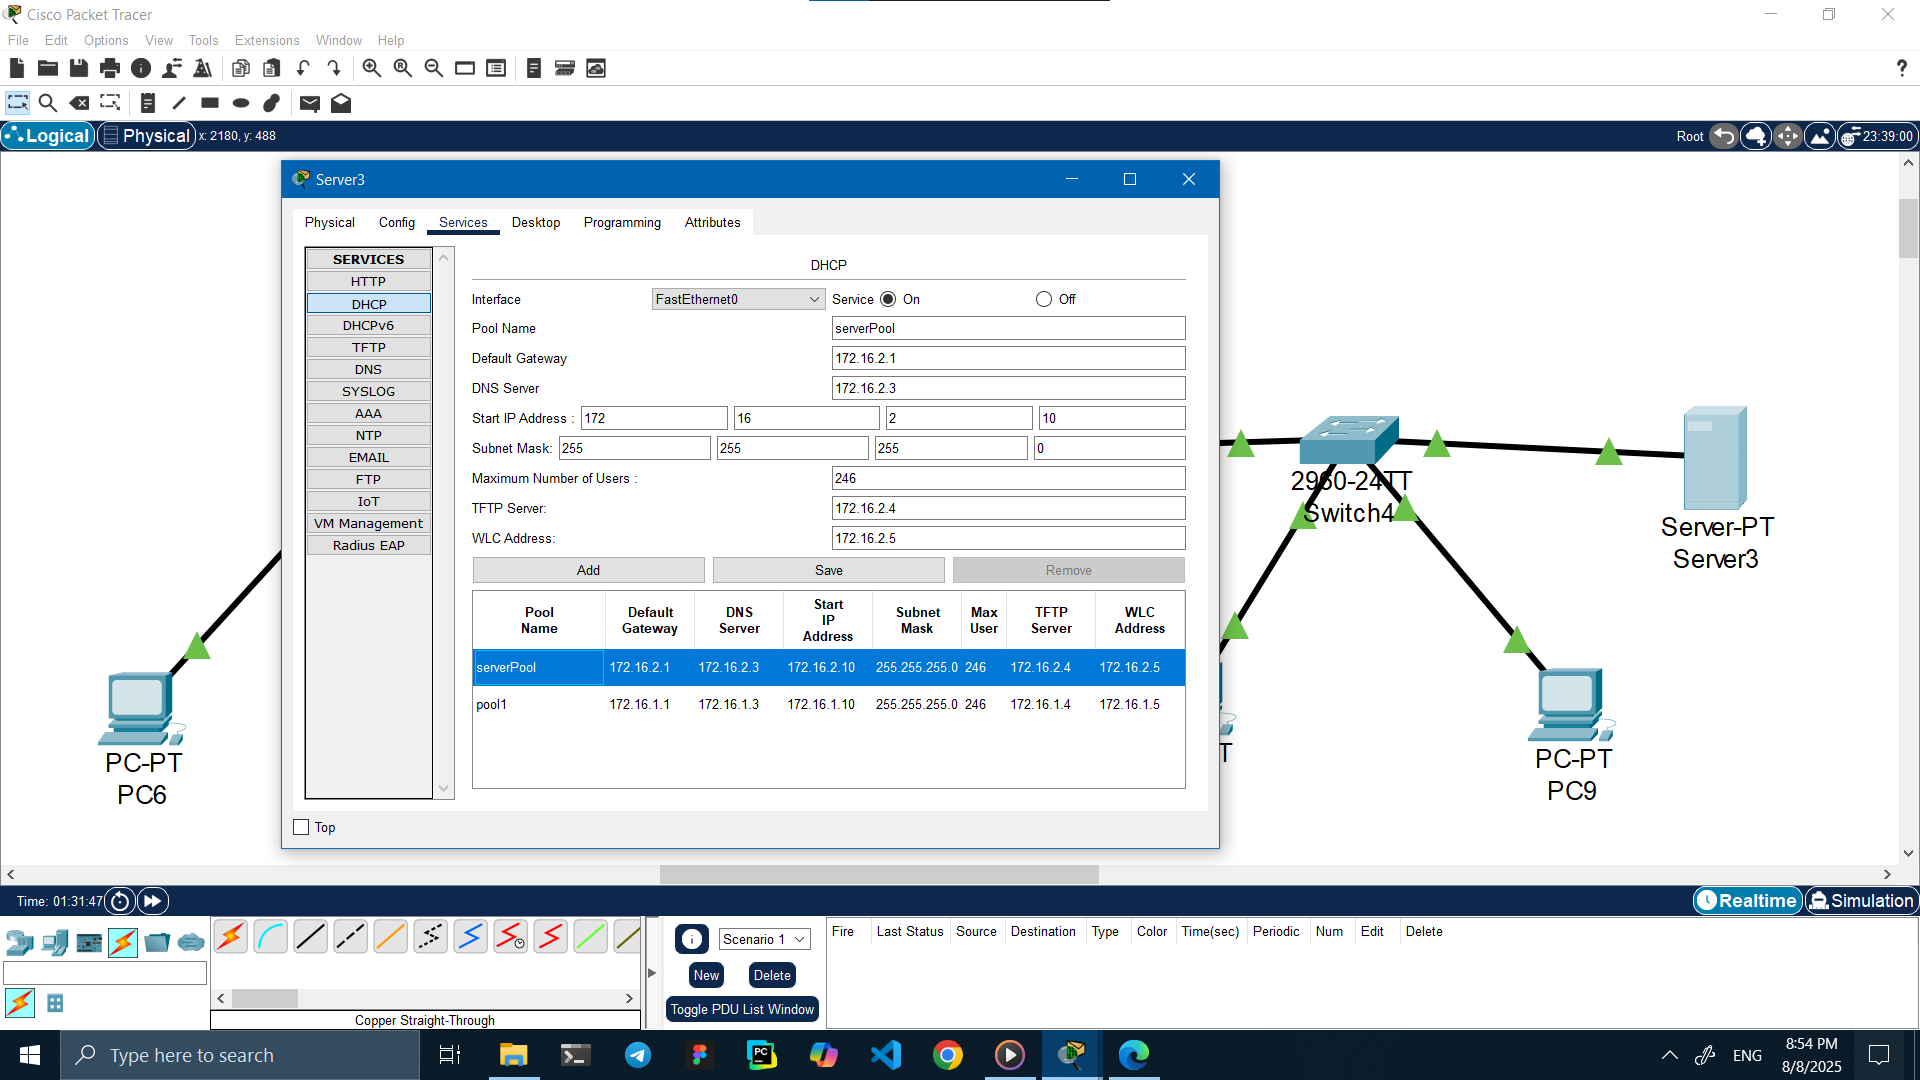
\includegraphics[width=\textwidth]{resources/scenario2-10.png}
		\caption{تنظیم سرویس \textenglish{DHCP} روی سرور و ایجاد دو \textenglish{pool} برای دو زیرشبکه‌ای که می‌خواهیم به آنها خدمات بدهیم}
		\label{2:10}
	\end{figure}
	\begin{figure}[H]
		\centering
		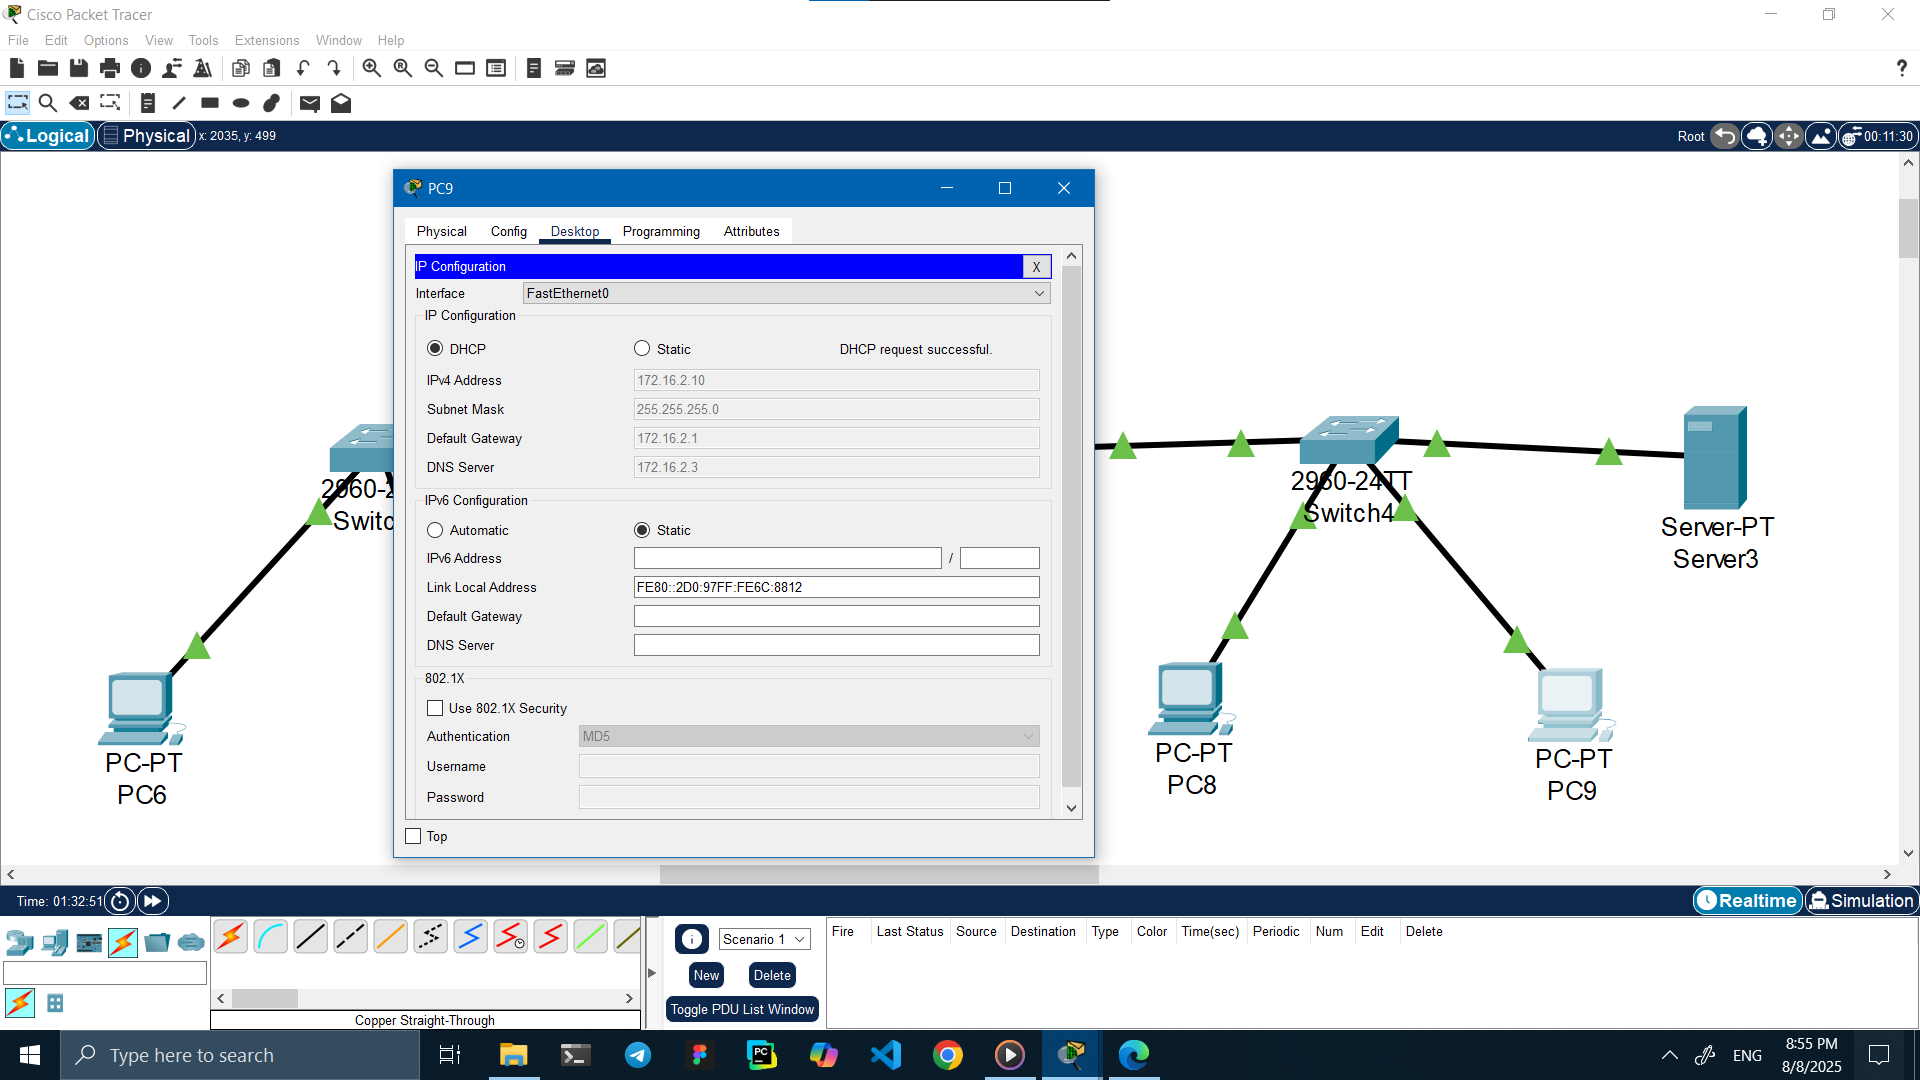
\includegraphics[width=\textwidth]{resources/scenario2-11.png}
		\caption{دریافت موفق آدرس \textenglish{ip} با \textenglish{DHCP} در یک \textenglish{PC} در همان شبکهٔ \textenglish{DHCP Server}}
		\label{2:11}
	\end{figure}
	\begin{figure}[H]
		\centering
		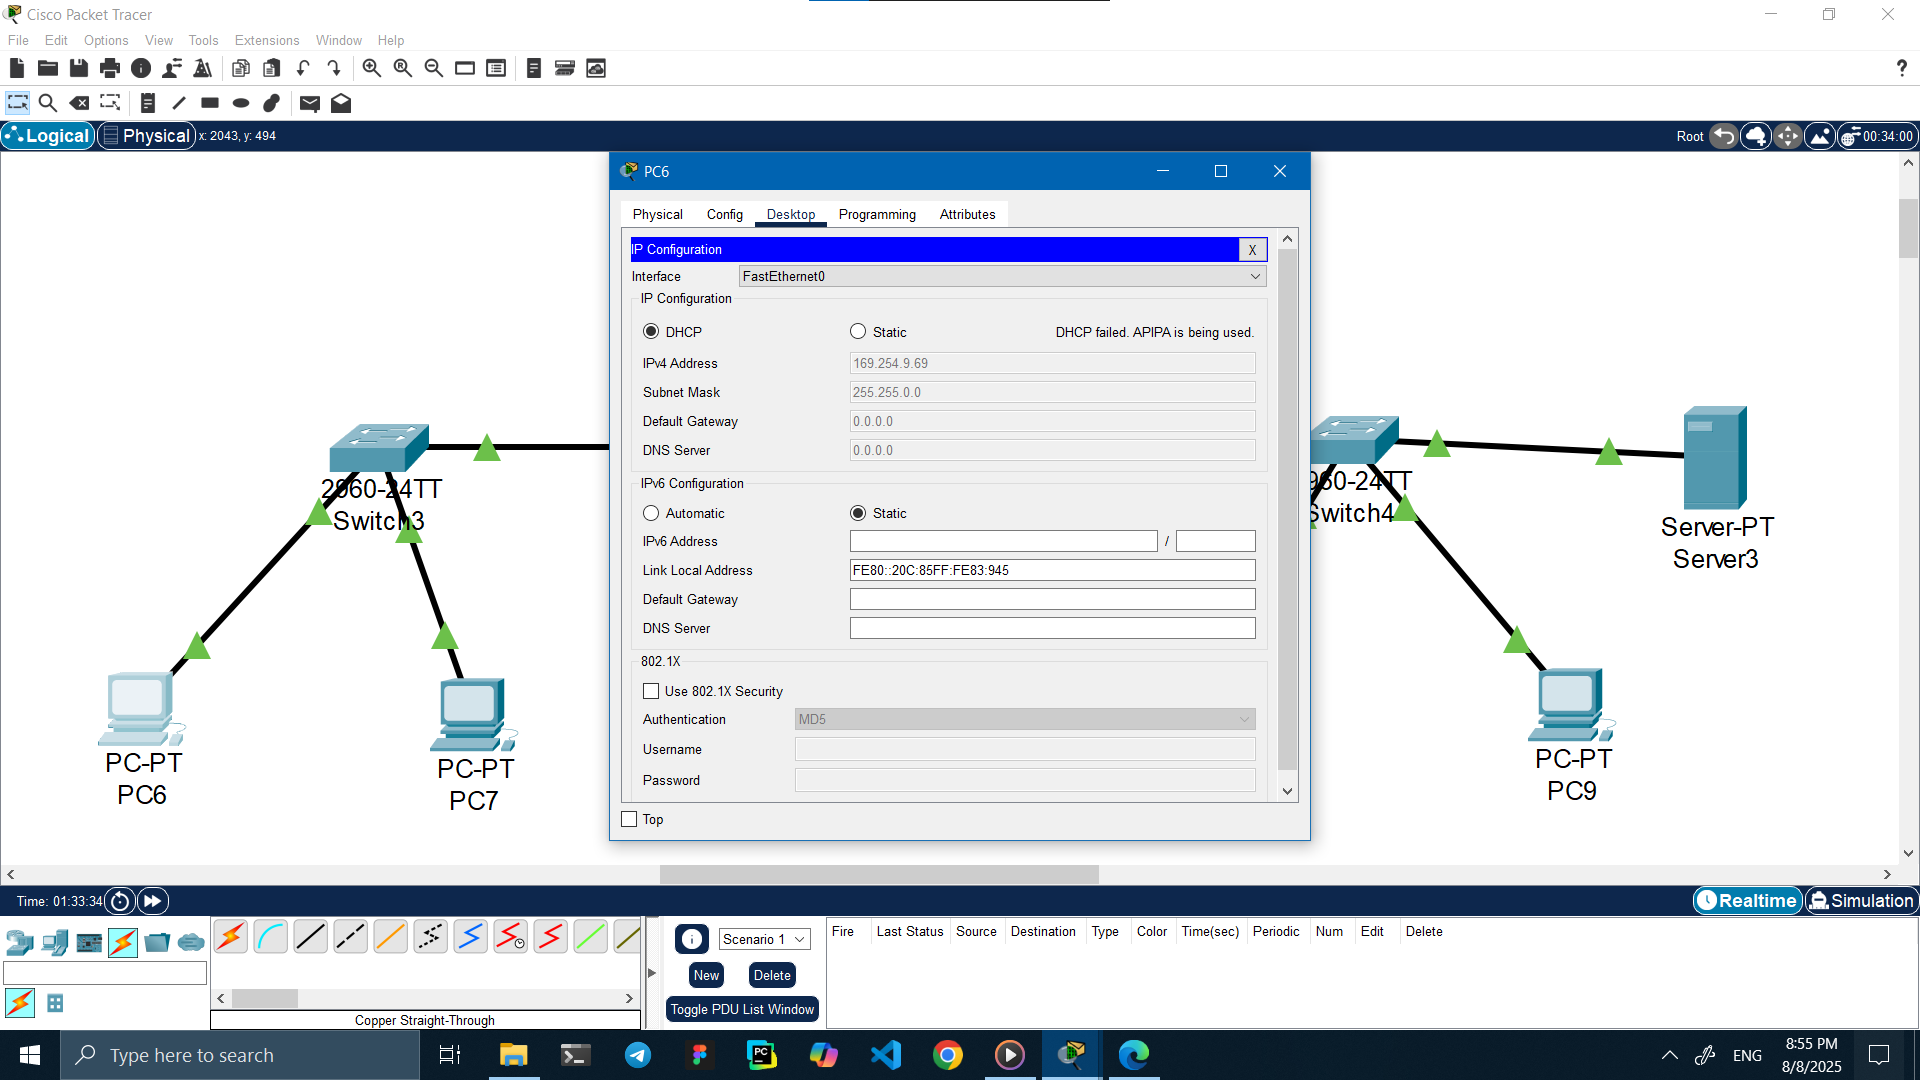
\includegraphics[width=\textwidth]{resources/scenario2-12.png}
		\caption{دریافت ناموفق آدرس \textenglish{ip} با \textenglish{DHCP} در یک \textenglish{PC} که در همان شبکهٔ \textenglish{DHCP Server} نیست}
		\label{2:12}
	\end{figure}
	\begin{figure}[H]
		\centering
		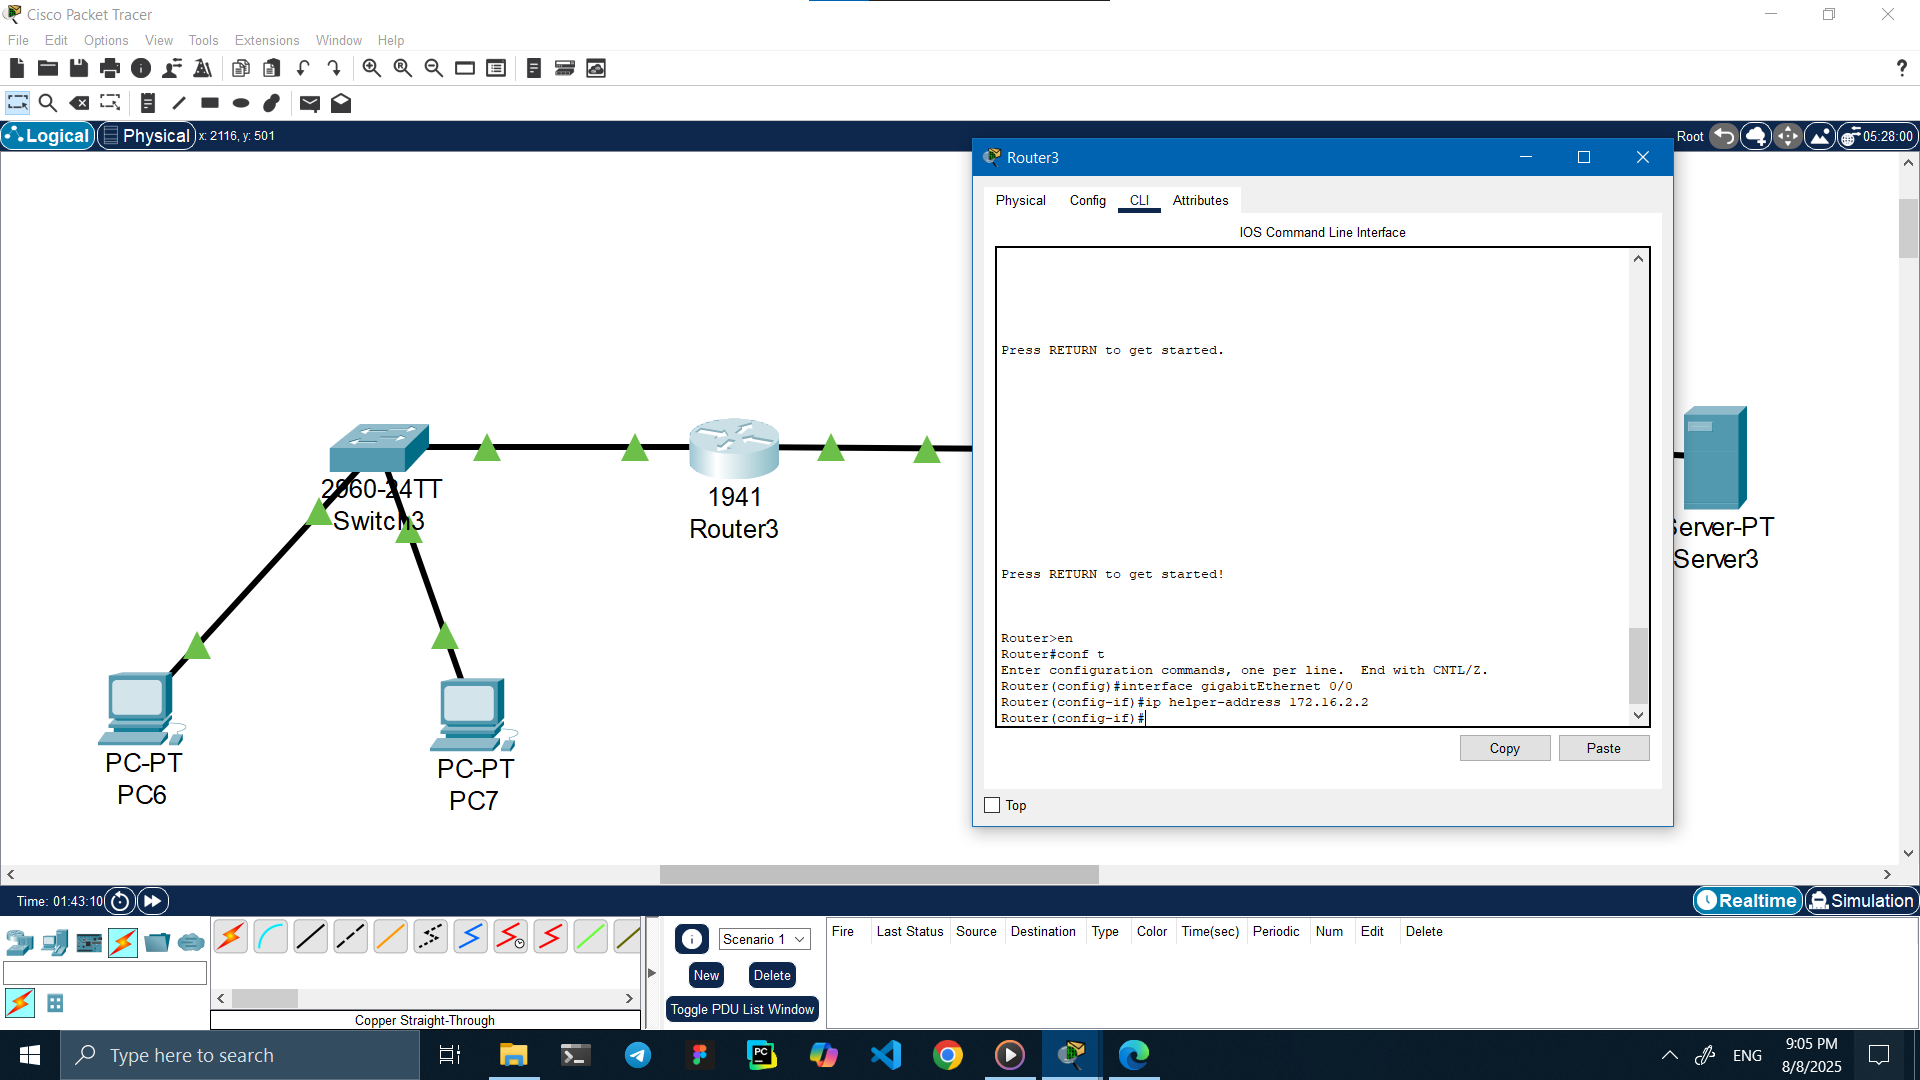
\includegraphics[width=\textwidth]{resources/scenario2-13.png}
		\caption{وارد کردن دستور \textenglish{ip helper-address} در روتر سمت چپ برای جلوگیری از افتادن بسته‌های \textenglish{broadcast} در مراحل \textenglish{DHCP}}
		\label{2:13}
	\end{figure}
	\begin{figure}[H]
		\centering
		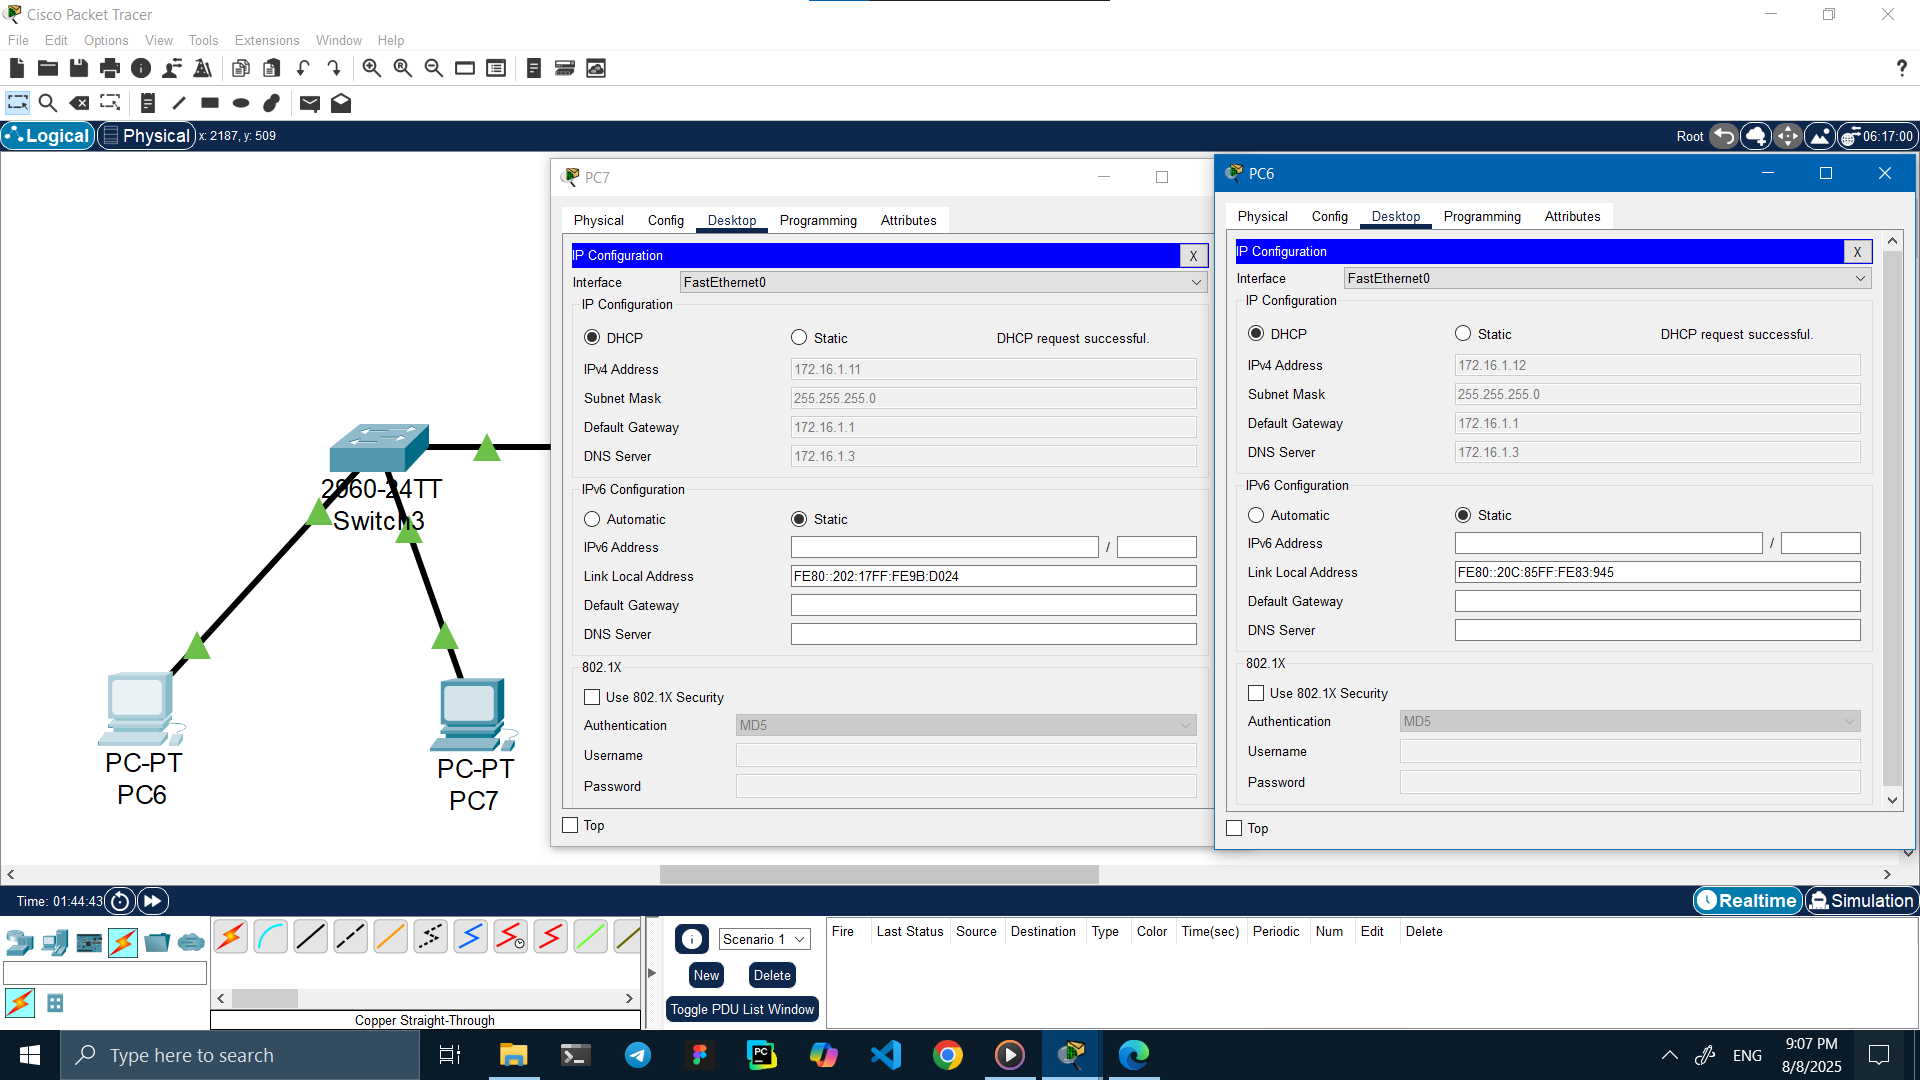
\includegraphics[width=\textwidth]{resources/scenario2-14.png}
		\caption{تخصیص درست آدرس به \textenglish{PC}‌های شبکه سمت چپ بعد از اعمال تنظیمات}
		\label{2:14}
	\end{figure}
	\newpage
	\section{سناریو ۳}
	در ابتدا دو مسیریاب و اتصال آنها را مانند شکل \ref{3:1} درست می‌کنیم. در ادامه برای مسیر‌یاب سمت راست که سرور است آدرس اضافه می‌کنیم و آن را روشن می‌کنیم. این کار در شکل \ref{3:2} انجام شده است. حالا باید در این سرور استخر‌ مناسب را اضافه کنیم و سرویس \textenglish{DHCP} را راه‌اندازی کنیم. شکل \ref{3:3} این موضوع را نشان‌ می‌دهد. حالا اگر بدون کار دیگری مسیریاب سمت چپ را بررسی کنیم، مطابق شکل \ref{3:4} می‌بینیم آدرس اختصاص داده نشده است. برای رفع این مشکل باید مطابق شکل \ref{3:5} به مسیریاب سمت چپ بگوییم که از \textenglish{DHCP} استفاده کند. حالا اگر دوباره مسیریاب را بررسی کنیم، مطابق شکل \ref{3:6} آدرس و مسیر به درستی داده شده است.
	\begin{figure}[H]
		\centering
		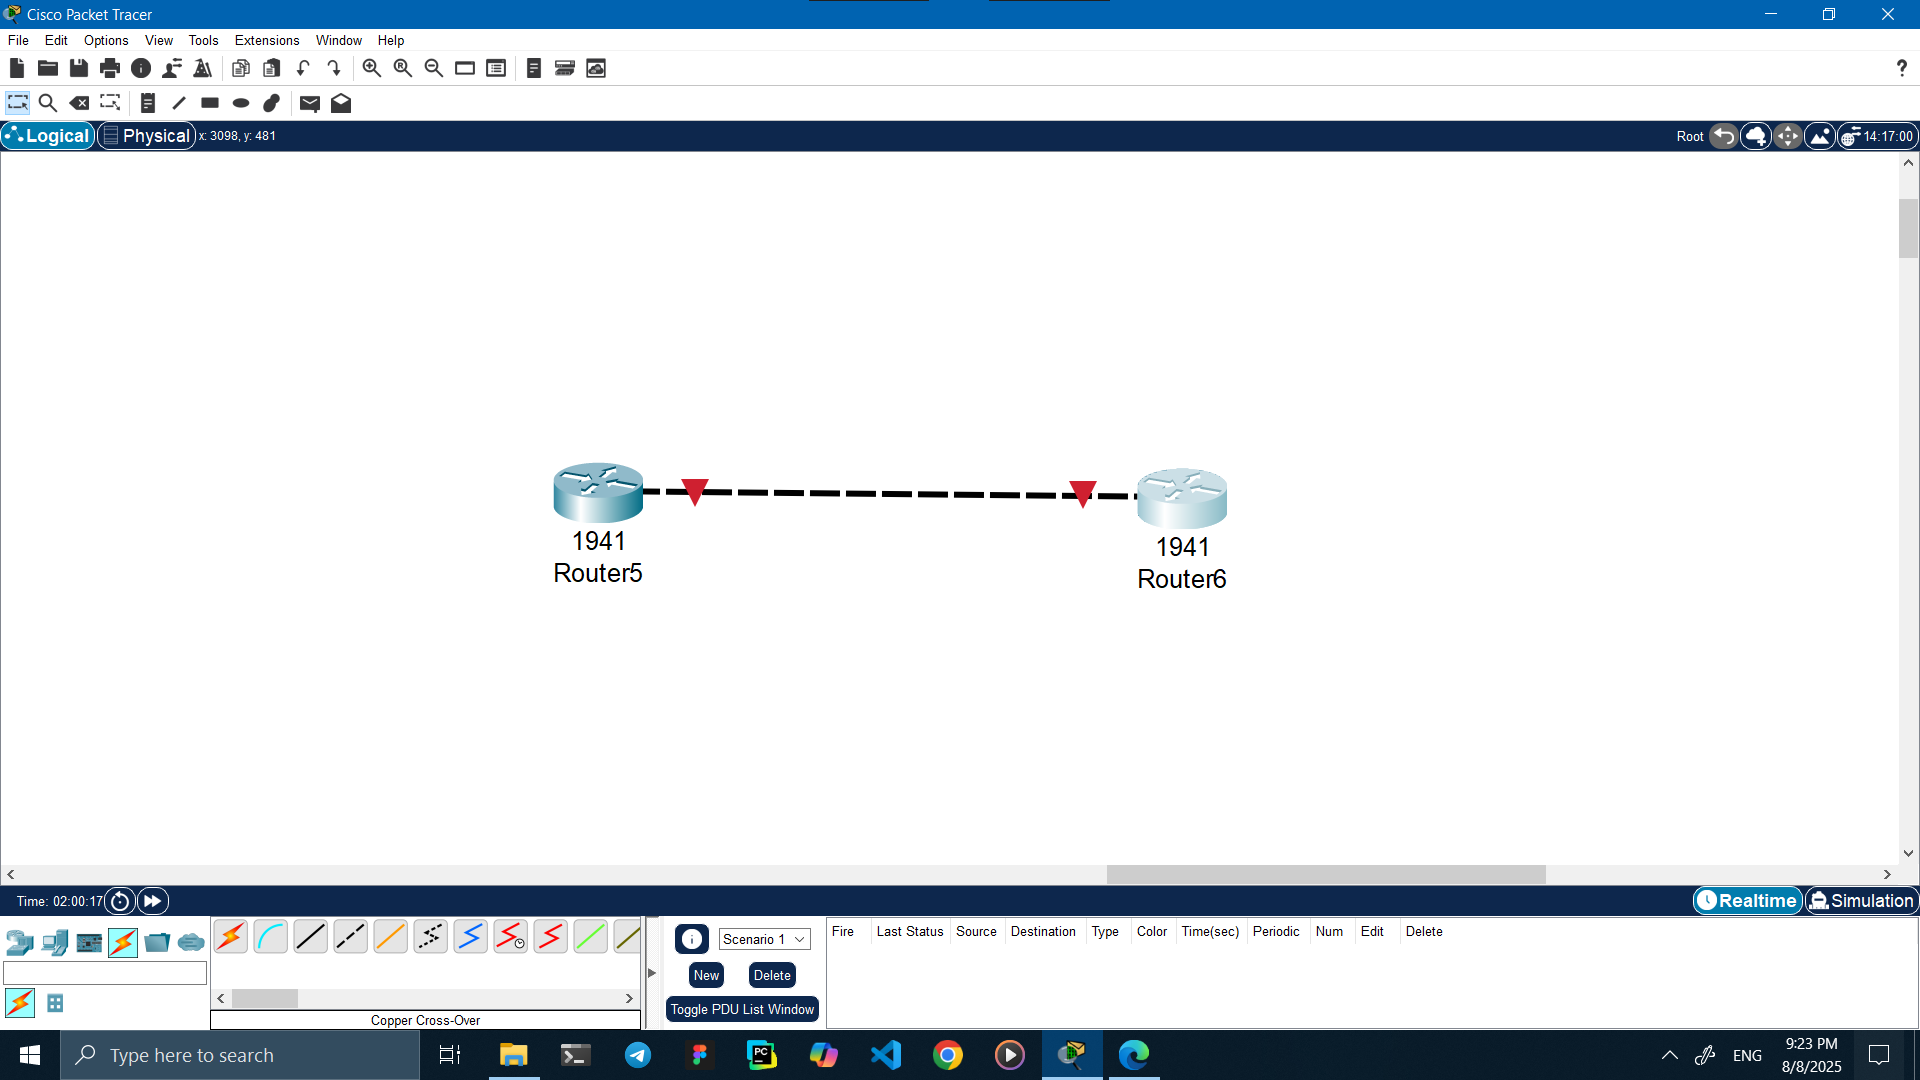
\includegraphics[width=\textwidth]{resources/scenario3-1.png}
		\caption{اضافه کردن دستگاه‌ها و اتصالات سناریو ۳}
		\label{3:1}
	\end{figure}
	\begin{figure}[H]
		\centering
		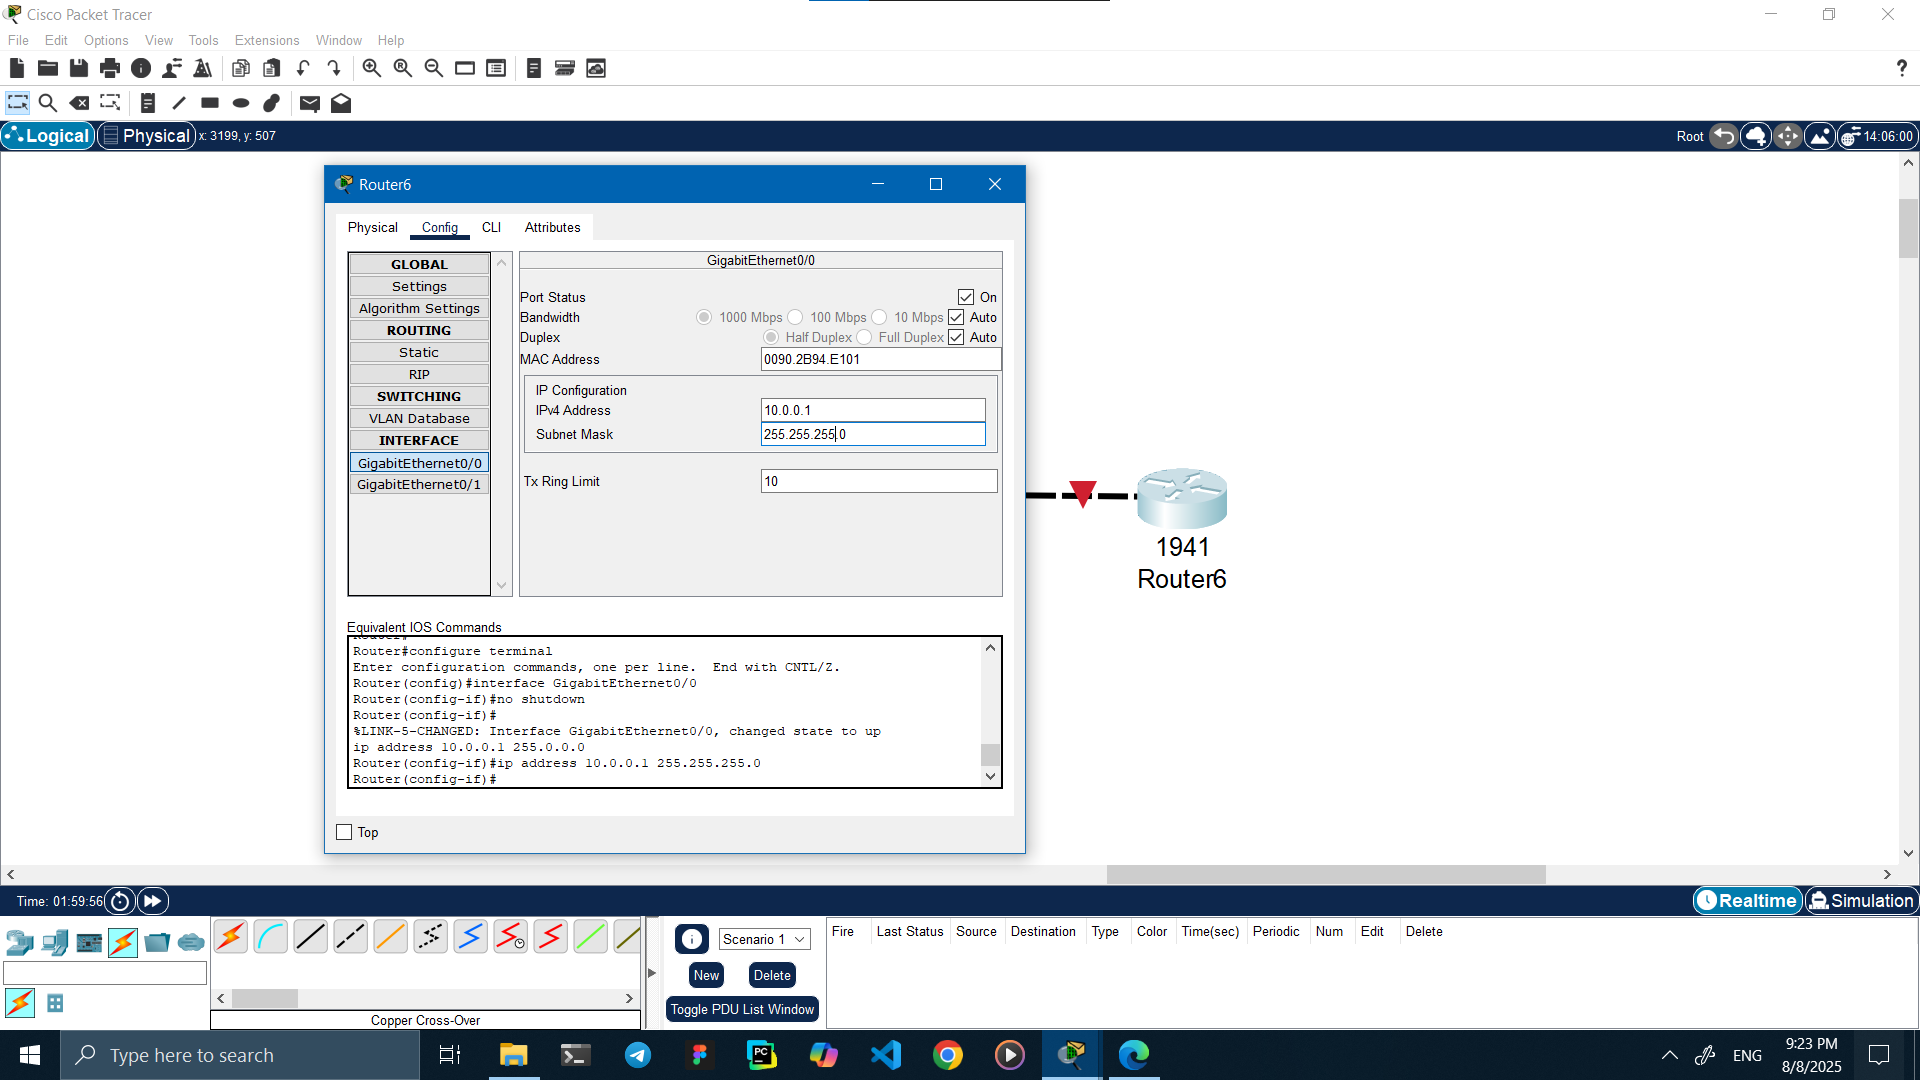
\includegraphics[width=\textwidth]{resources/scenario3-2.png}
		\caption{تنظیم آدرس \textenglish{ip} سرور (\textenglish{Router} سمت راست) و اطمینان از روشن بودن آن}
		\label{3:2}
	\end{figure}
	\begin{figure}[H]
		\centering
		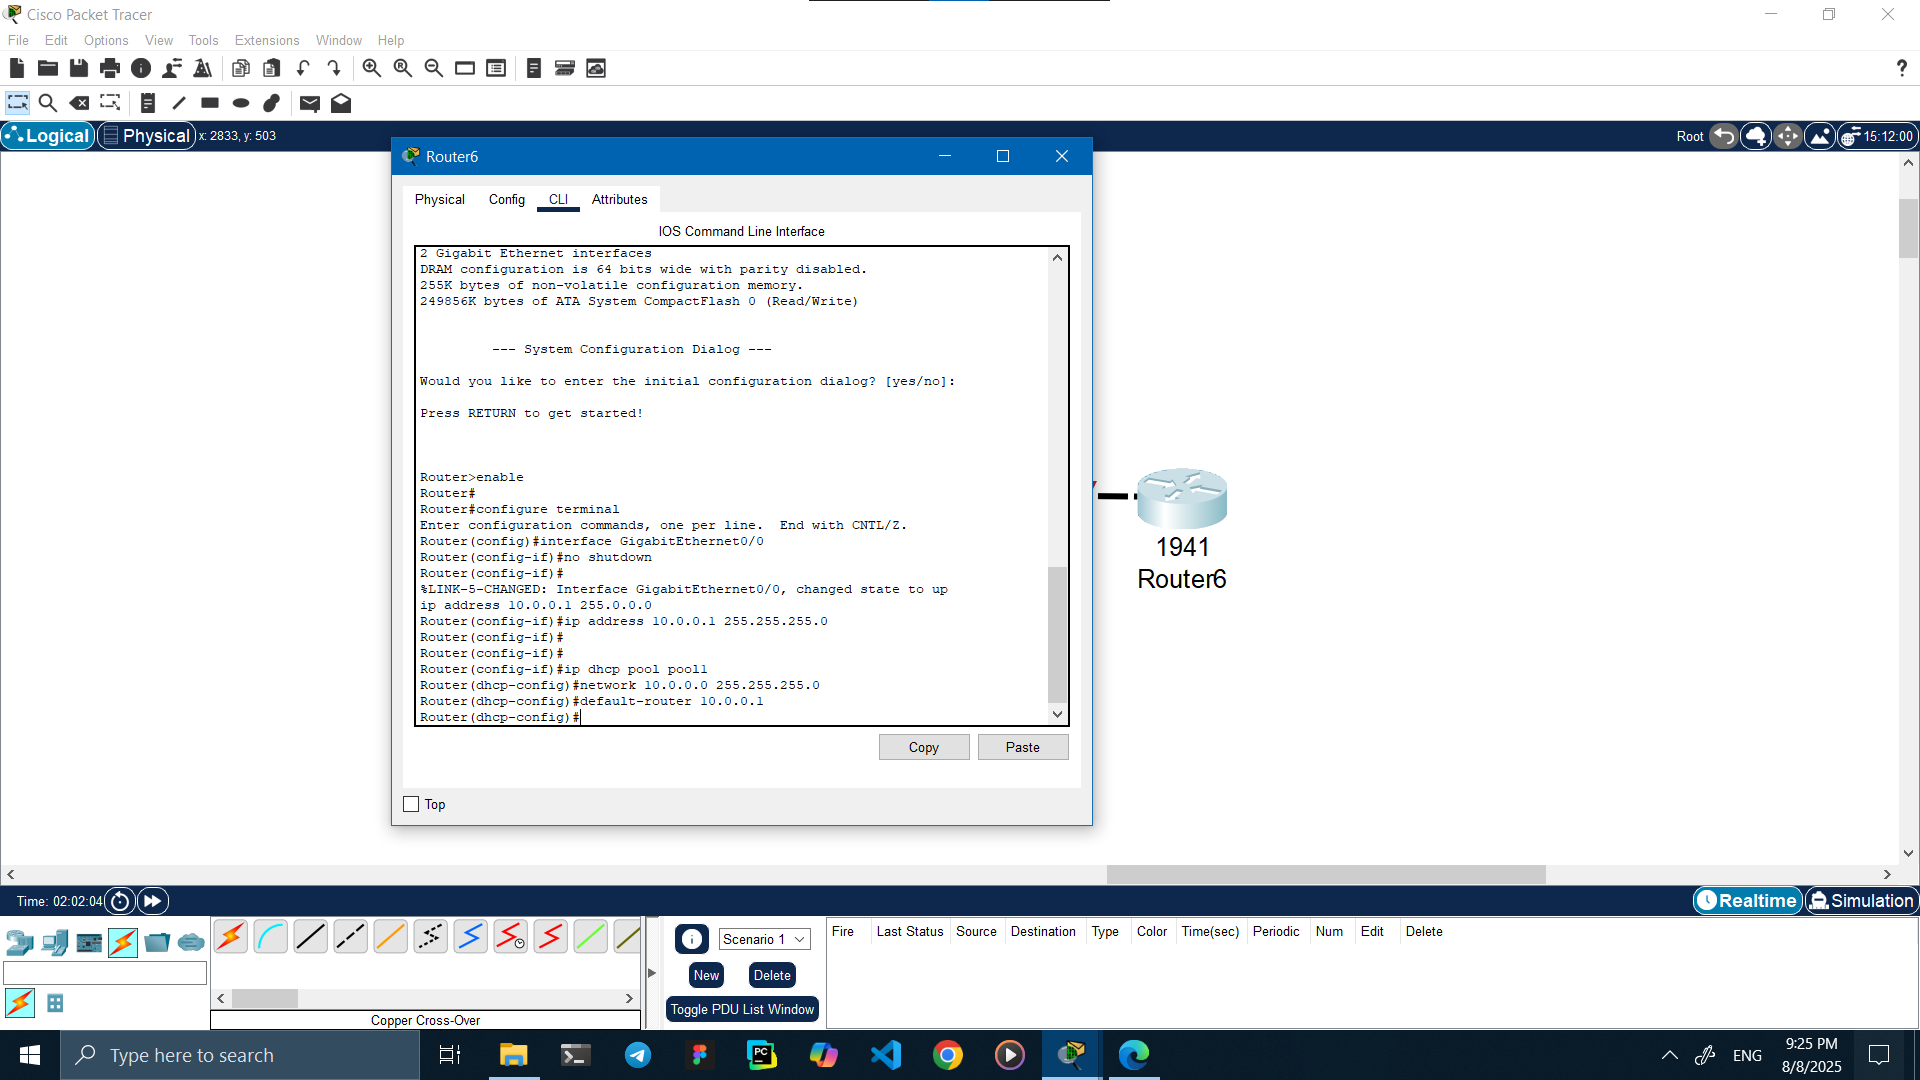
\includegraphics[width=\textwidth]{resources/scenario3-3.png}
		\caption{ایجاد \textenglish{pool} مناسب در \textenglish{Router} سرور برای خدمت \textenglish{DHCP}}
		\label{3:3}
	\end{figure}
	\begin{figure}[H]
		\centering
		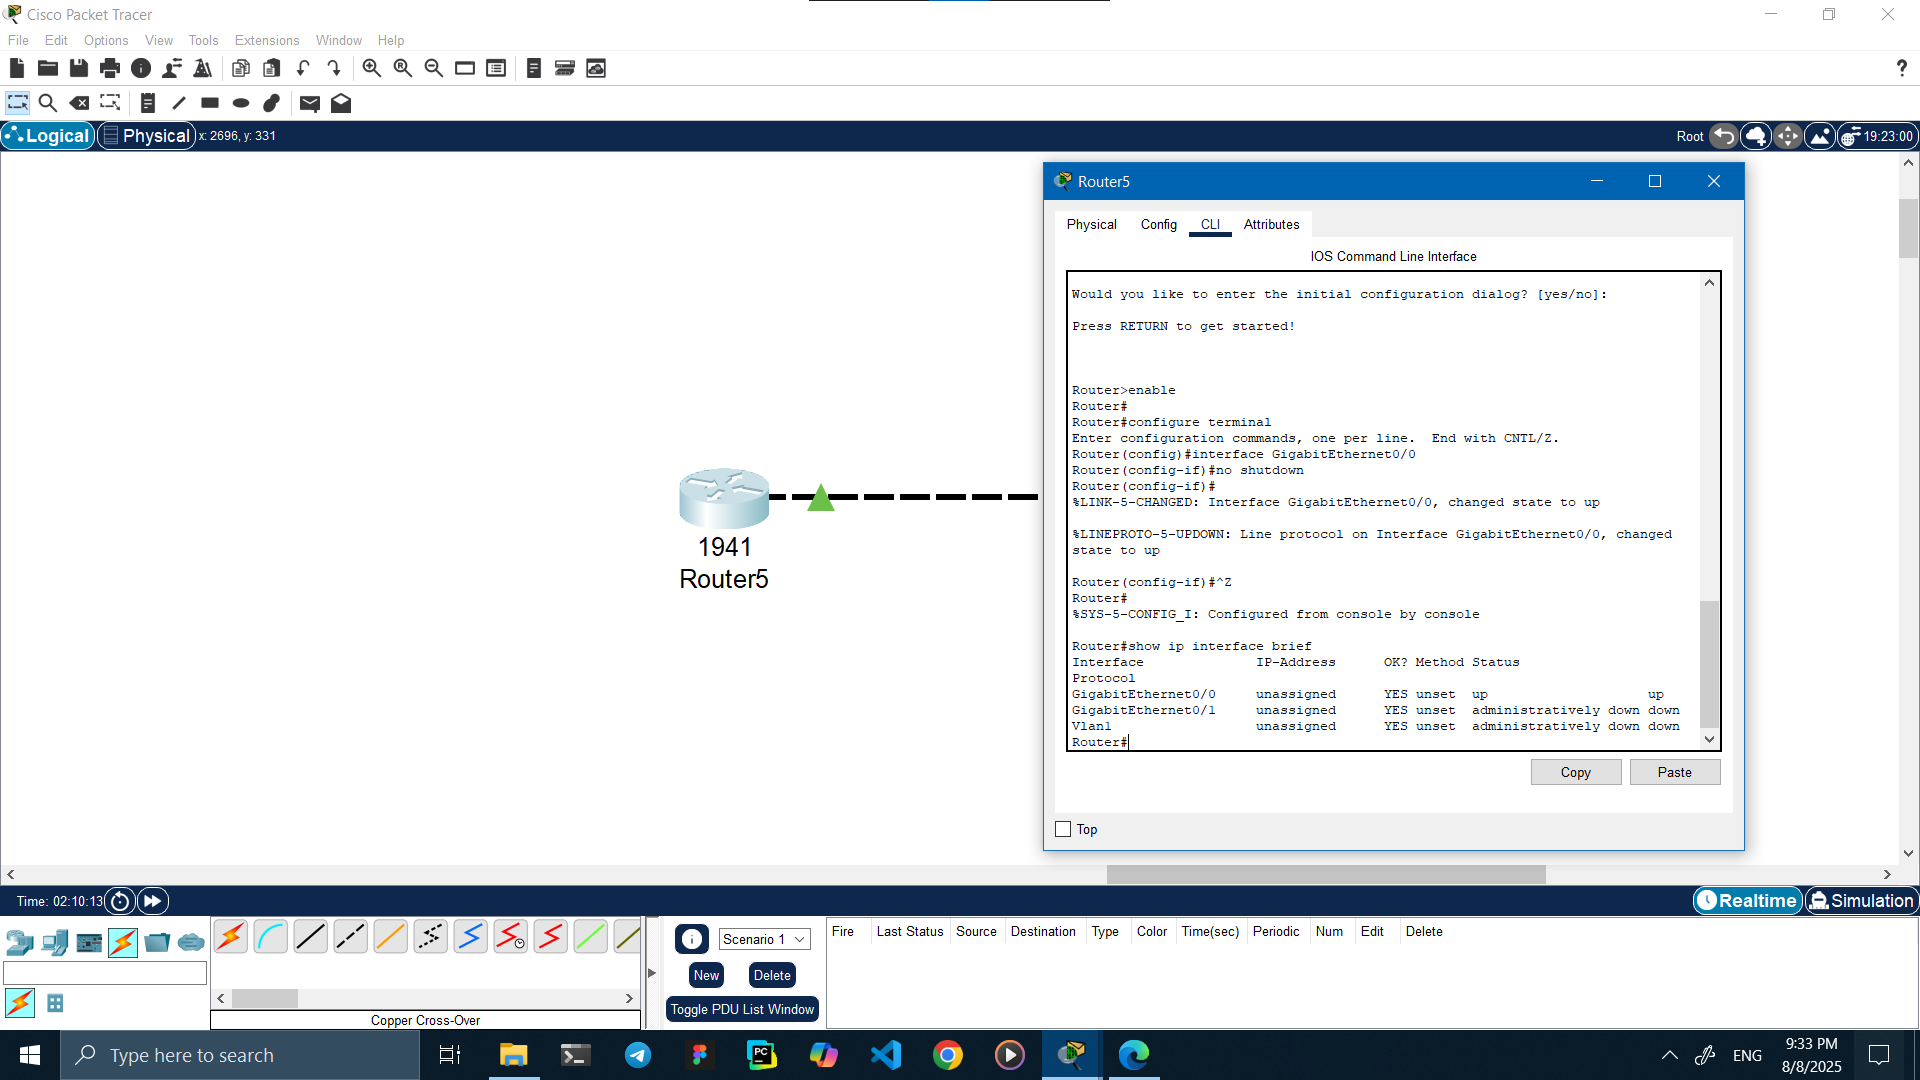
\includegraphics[width=\textwidth]{resources/scenario3-4.png}
		\caption{\textenglish{Router} سمت چپ در ابتدا آدرسی ندارد}
		\label{3:4}
	\end{figure}
	\begin{figure}[H]
		\centering
		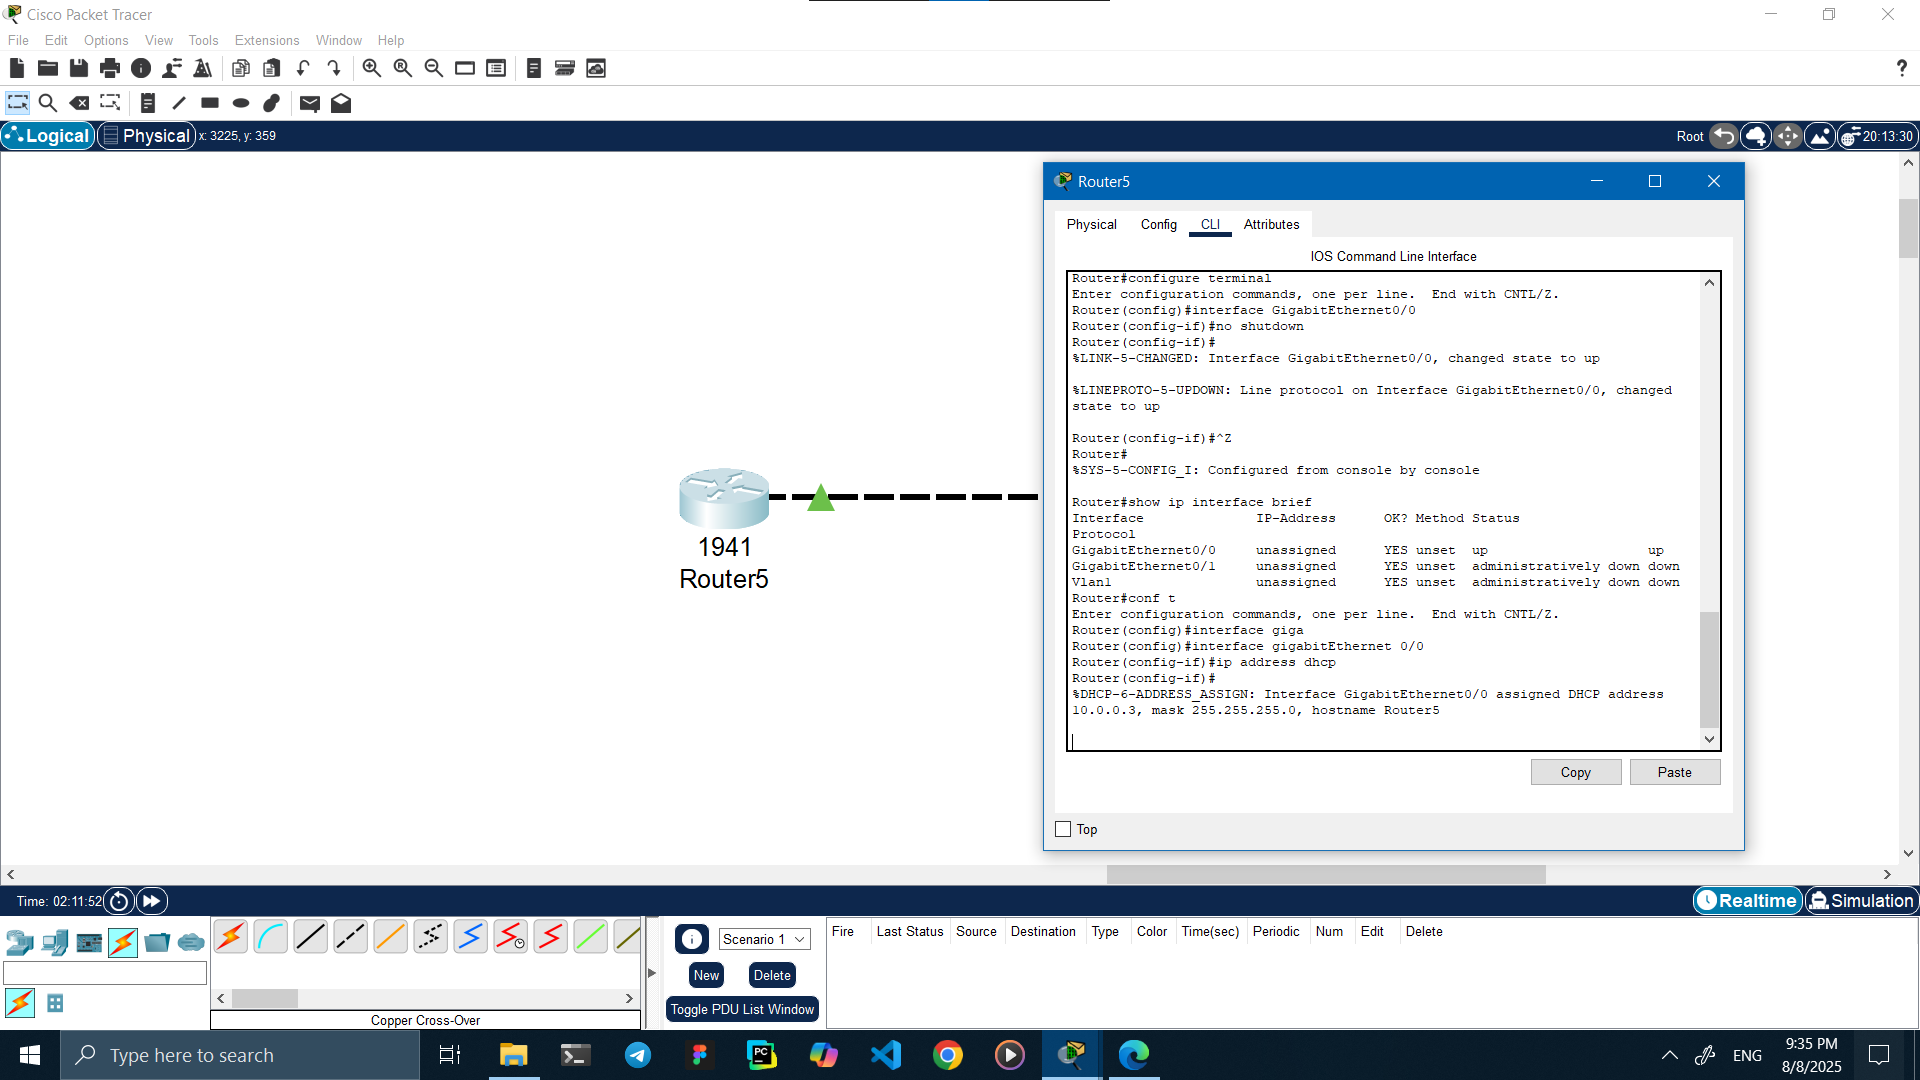
\includegraphics[width=\textwidth]{resources/scenario3-5.png}
		\caption{تنظیم نحوه دریافت آدرس در \textenglish{Router} سمت چپ با \textenglish{DHCP} و پیام دریافت آدرس از سرور}
		\label{3:5}
	\end{figure}
	\begin{figure}[H]
		\centering
		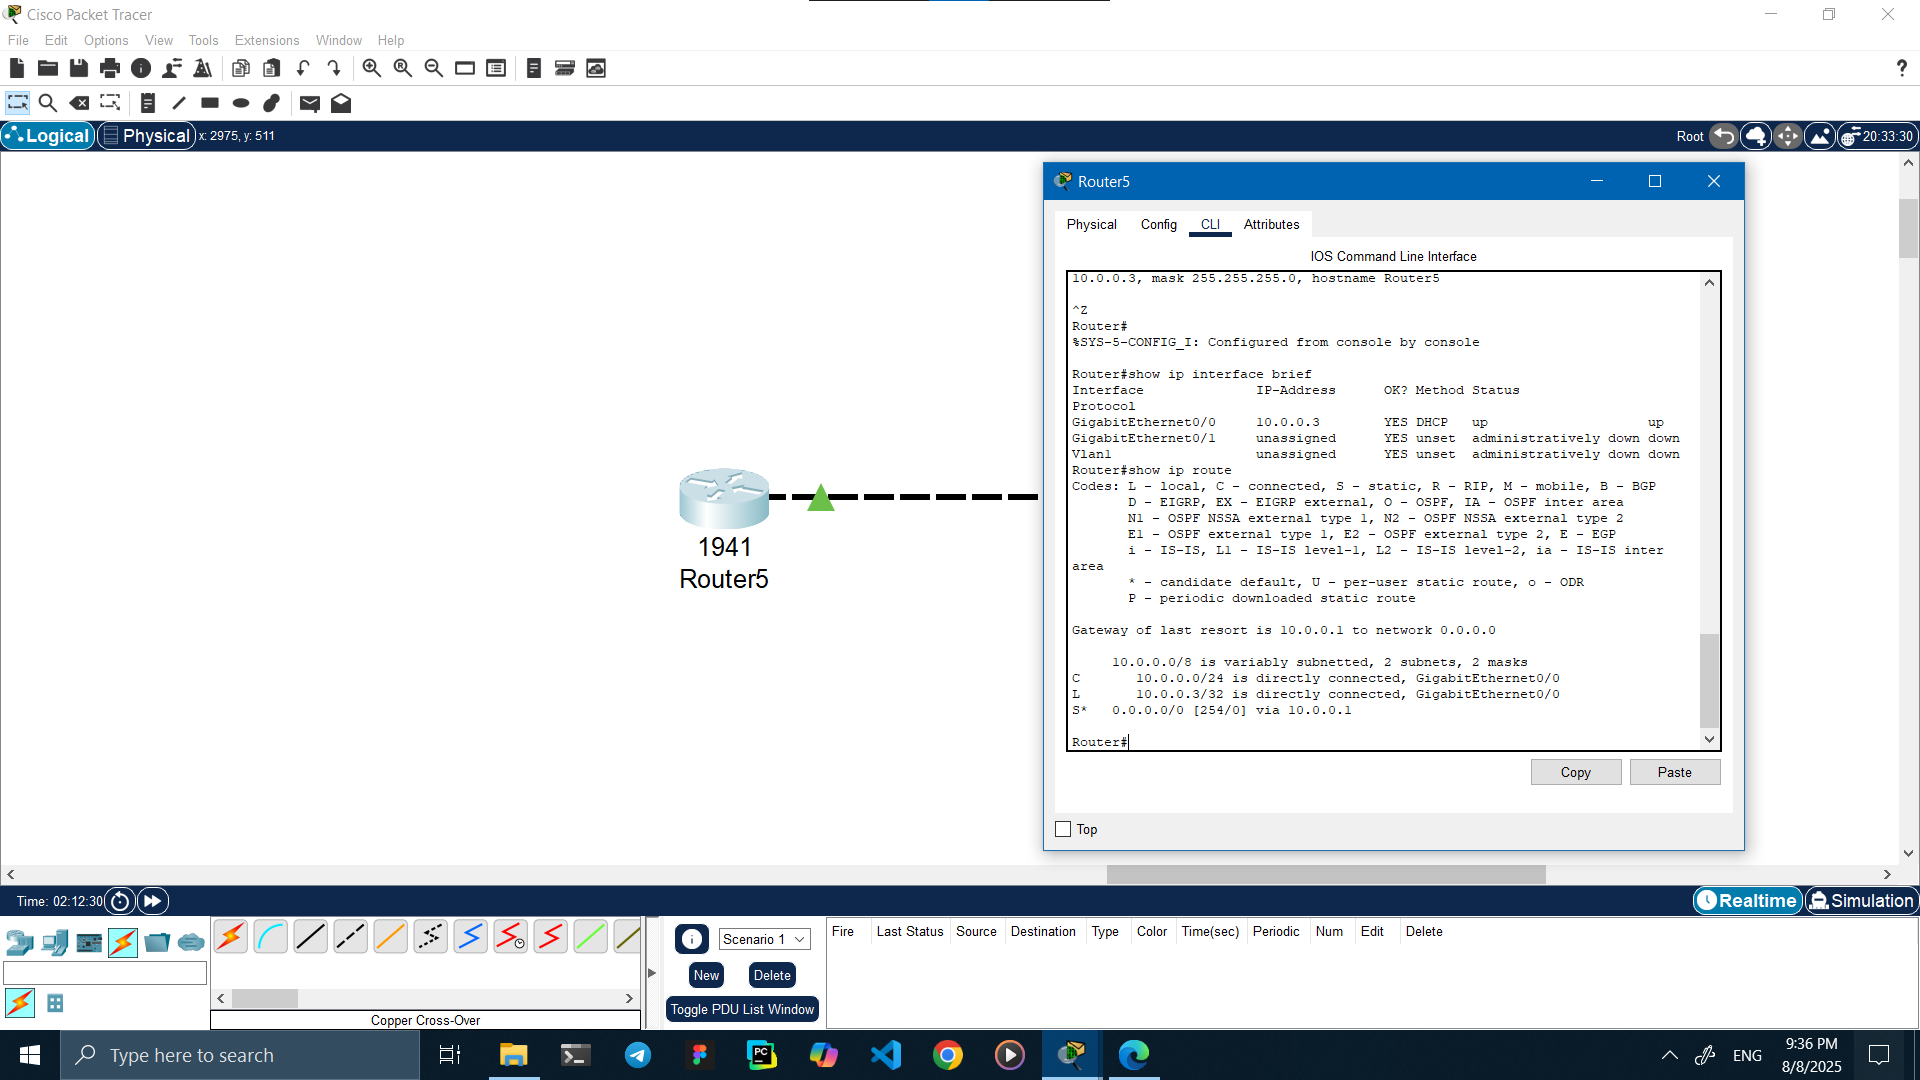
\includegraphics[width=\textwidth]{resources/scenario3-6.png}
		\caption{مشاهده اختصاص موفق آدرس با \textenglish{DHCP}}
		\label{3:6}
	\end{figure}
	
	% ==============================
	% References
	% ==============================
	\newpage
	\begin{LTR}
		\printbibliography[title={مراجع}]
	\end{LTR}
	
\end{document}
